\chapter{Background Research and Literature Review}

In Information Security, anonymity can be a difficult notion to conceptualize. This chapter begins by introducing two different aspects of anonymity so as to place this study in context. Next, it follows an in depth description of the Dining Cryptographers protocol, the main focus of the thesis, starting from a theoretical standpoint and ending with practical considerations for the suggested implementation. Lastly, the chapter will outline the current state of art of DC-Net implementations.

\section{What is Anonymity}
Generally speaking, the definition of anonymity is presented as a "lack of outstanding, individual, or unusual features." \cite{Anonymity}. In Information Security, anonymity is a security goal a system may want to achieve. Attaining such security property means that it is infeasible to hold a principal accountable for an anonymous action. In other words, anonymity prevents any principal from identifying another principal performing an action within an anonymous network \cite{Malkhi}.

An anonymity network composed of a finite set of participants is called anonymity set.

\subsection{Anonymity Set} \label{sec:anonymityset}
When considering an anonymity set, anonymity is precisely defined in relation to others: for a principal to be anonymous in doing an action, other subjects An anonymity network composed of a finite set of participants is called anonymity set \cite{Pfitzmann}.

It follows that the number of agents inside the anonymity set determines the level of anonymity that can be achieved. Therefore, anonymity is an incremental concept: the more the participants inside an anonymous network, the higher the degree of anonymity. The minimum number of principals to guarantee this property is two,as a network with one agent exhibits no anonymity whatsoever (See Figure \ref{fig:anonymity}) \cite{Franck}.

\begin{figure}[h]
    \centering
    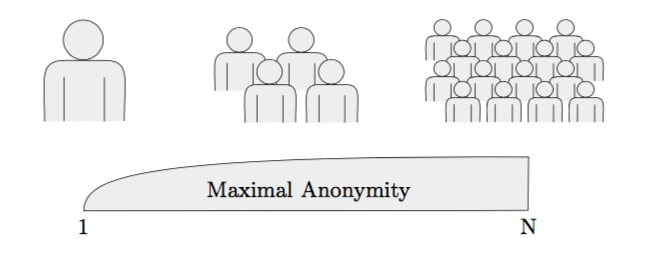
\includegraphics[width=0.50\textwidth]{Images/anonymityLevel.png}
    \caption{Level of anonymity in a set \cite{Franck}}
    \label{fig:anonymity}
\end{figure}

The features of anonymity presented above fit well with the definition of 'hiding one's identity'. 
In information security, however, considering the types of anonymity set adds another dimension to the concept. There are two types of anonymity set: sender anonymity set and recipient anonymity set. The former refers to multiple participants inside the set of senders and one, or possibly more, agents in the recipients set (figure \ref{fig:senderAnonSet}). The latter, instead, refers to the opposite scenario having many recipients in one set and one, or possibly more, senders in the other (figure \ref{fig:receipientAnonSet}).


\begin{figure}[h]
\centering
\begin{minipage}{.5\textwidth}
    \centering
    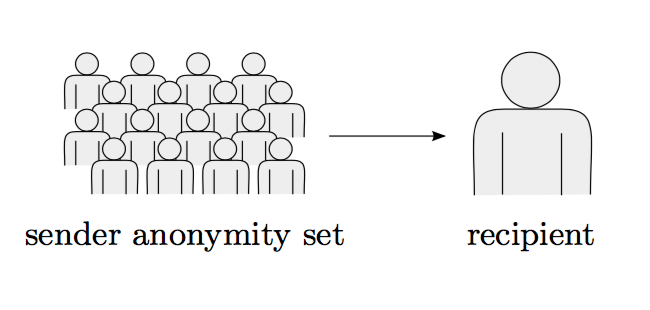
\includegraphics[width=0.50\textwidth]{Images/ReceiverAnonymSet.png}
    \caption{Sender anonymity set \cite{Franck}}
    \label{fig:senderAnonSet}
\end{minipage}%
\begin{minipage}{.5\textwidth}
    \centering
    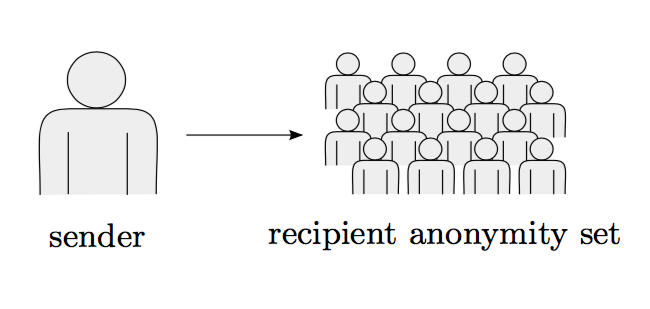
\includegraphics[width=0.50\textwidth]{Images/senderAnonymSet.png}
    \caption{Recipient anonymity set \cite{Franck}}
    \label{fig:receipientAnonSet}
\end{minipage}
\end{figure}



\begin{figure}[h]
    \centering
    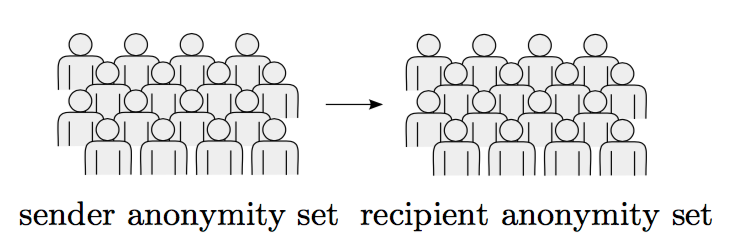
\includegraphics[width=0.50\textwidth]{Images/ManyToManyAnonymSet.png}
    \caption{Anonymity sets with multiple senders and recipients \cite{Franck}}
    \label{fig:anonymityLevel}
\end{figure}

Senders and recipients may overlap in the same set as shown in figure \ref{fig:overlappingAnonSet}.

\begin{figure}[h]
    \centering
    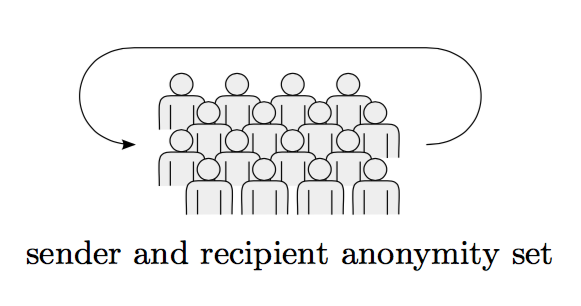
\includegraphics[width=0.50\textwidth]{Images/overlappingAnonymSet.png}
    \caption{Overlapping senders and receivers in anonymity set \cite{Franck}}
    \label{fig:overlappingAnonSet}
\end{figure}


\subsection{Identity Anonymity versus Sender/Recipient Anonymity}
When considering what anonymity means in the two types of anonymity set, the notion shifts from a participant's identity being hidden to being untraceable, i.e. an action cannot be traced back to a specific principal within the set. In fact, all senders identities and/or recipients identities can be known. However, if a principal would like to perform an action - like sending a message - all other participants also perform the same action - in this case act as senders by dispatching a dummy messages (noise) - so that it is not distinguishable which of all the messages is the real message and, as a consequence, who is the real sender.

As a result of this analysis, it follows that the classic notion of anonymity refers to hiding one's identity. However, a different concept is sender/recipient anonymity, which instead equates to the concept of untraceability. Specifically, untraceability has as its main feature the inability of determine which principal of the network, with  knowable identities, is the actual sender or recipient of a message. \newline 


In this frame of reference, the Dining Cryptographer protocol is a protocol that offers strong sender and recipient untraceability \cite{Chaum}, which is the central subject of this thesis. Therefore, at least from a theoretical standpoint, in a Dining Cryptographers Network senders and recipients are completely untraceable. 

The use of the term anonymity from now on in this document refers solely to sender/recipient anonymity, i.e. untraceability, unless explicitly stated otherwise.

\section{The Dining Cryptographers}
David Chaum first theorised this concept in "The Dining Cryptographers Problem" publication in the Journal of Cryptology in January 1988 (Volume 1, Issue 1, pp 65-75). Chaum here describes a protocol that employs one-time-use keys in order to offer unconditional sender and receiver untraceability within a network (a DC-Net) \cite{Chaum}. 

To simplify the understanding of the underlying techniques of the protocol to the reader, Chaum's analogy is presented first, followed by a more formal exposition.

\subsection{The protocol Analogy - The Dinner}
Three cryptographers decide to dine at a restaurant. At the end of the meal, the waiter informs the table that the bill has already been paid anonymously. The arrangement might have been made by one of the three dining cryptographers or by their employer, the National Security Agency (the NSA). The diners respect each other's privacy to pay anonymously, but they are interested to know if the payer is at the table or if indeed it was their employer. In order to determine the answer, they execute the following three phases \cite{Chaum}:
\begin{enumerate} \label{sec:protocolStages}
    \item Every cryptographer has one neighbour sitting on his left and one of his right. Each cryptographer tosses an unbiased coin behind a menu between him and his right neighbour so that the third participant cannot see the outcome (Figure \ref{fig:dcstage1}). At this point, each cryptographer can see the result of two coin flips, the one he flipped with his right neighbour and the one that his left neighbour flipped with him (Figure \ref{fig:dcstage2}). 
    \item Subsequently, each cryptographer states out loud whether the two coins have the same value (two heads or two tails) or otherwise (Figure \ref{fig:dcstage3}). If the cryptographer paid for the dinner, he lies about the result of the coins and says the exact contrary of what he sees.
    \item Finally, all the results of the three cryptographers are combined in order to find the truth about who paid. An even number of "Different" means that the NSA paid for the dinner, and odd number of "Different" means that one of the cryptographers at the table paid for the dinner.
\end{enumerate}

\begin{figure}[h!]
    \centering
    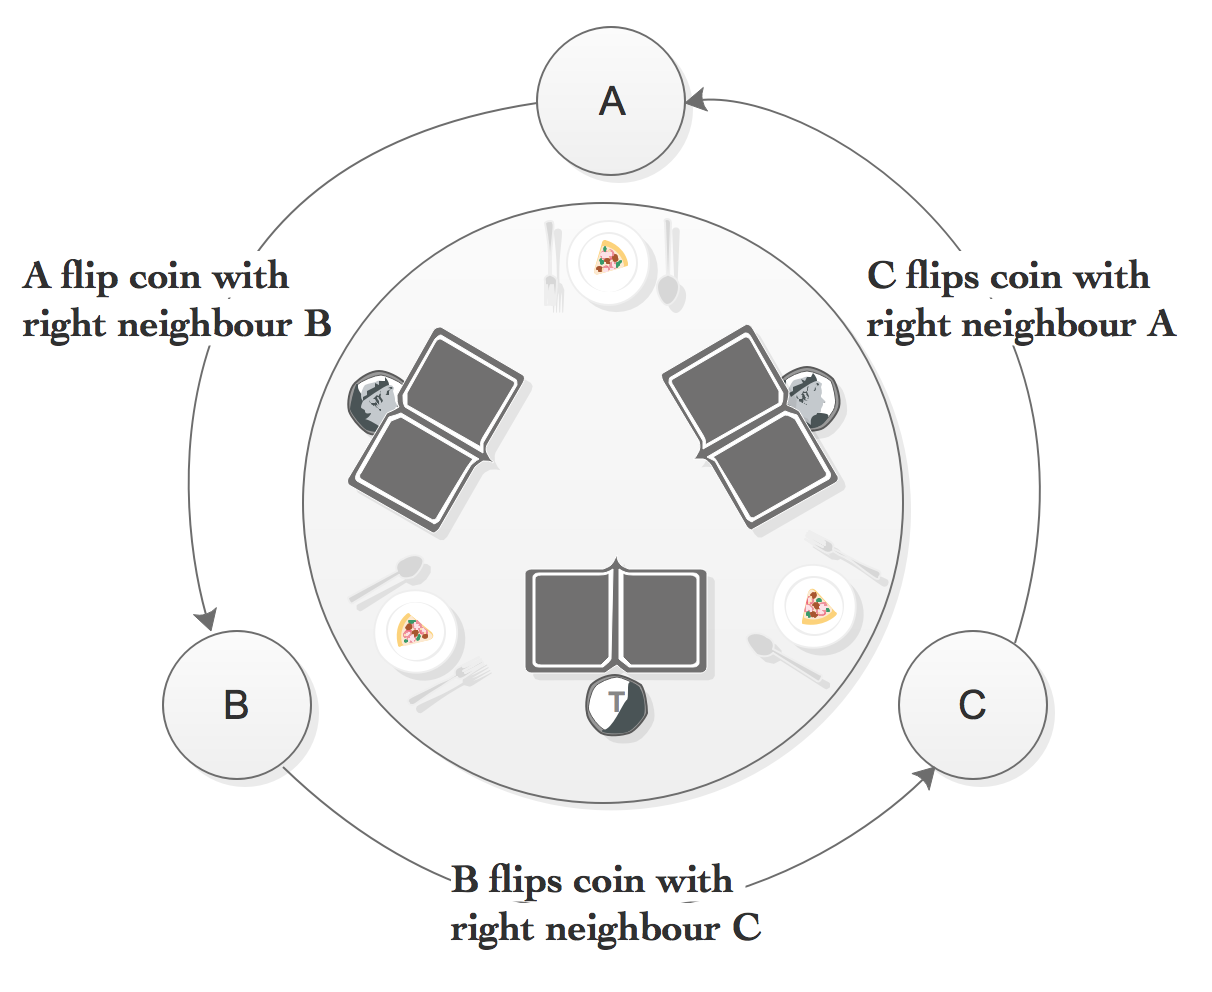
\includegraphics[width=0.50\textwidth]{Images/DCstep1.png}
    \caption{Diners flip coins}
    \label{fig:dcstage1}
\end{figure}

\begin{figure}[h!]
    \centering
    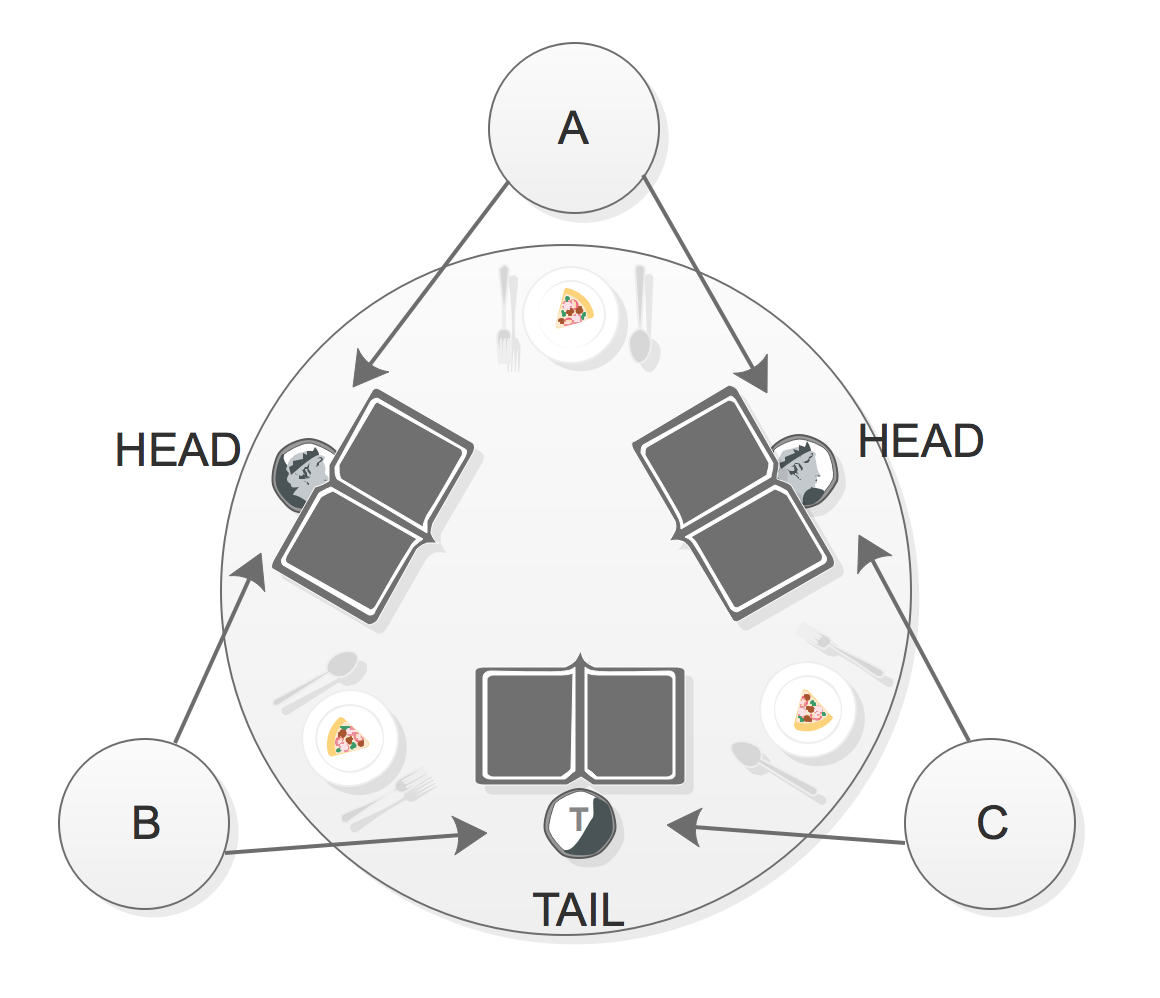
\includegraphics[width=0.50\textwidth]{Images/DCstep2.png}
    \caption{What each cryptographer can see}
    \label{fig:dcstage2}
\end{figure}

\begin{figure}[h!]
    \centering
    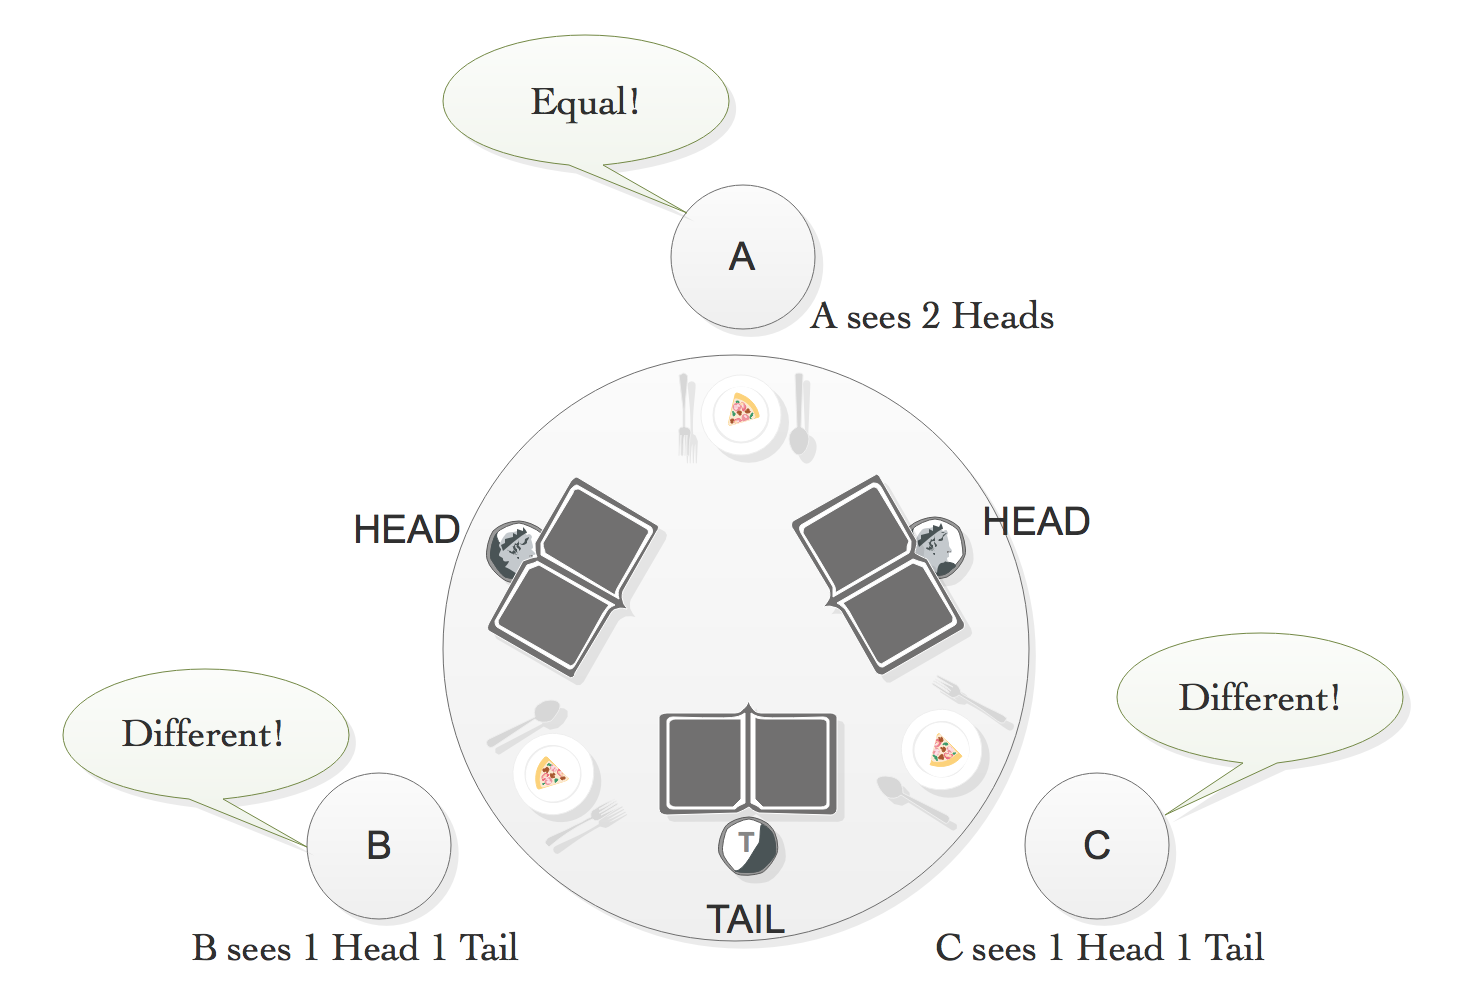
\includegraphics[width=0.70\textwidth]{Images/DCstep3NoPayers.png}
    \caption{Cryptographers broadcast responses. Even number of "Different" implies that no one is the payer.}
    \label{fig:dcstage3}
\end{figure}

To sum up, if one of the three cryptographers at the table paid for the meal, neither of the two non-paying cryptographers would gain any additional information about who, between the two other participants other than himself, might be the payer. This is because each participant does not know the outcome of the third coin flip between the other two participants.  Such is the explanation of how sender anonymity is guaranteed in the Dining Cryptographers protocol. 

Importantly, Chaum also proves how sender anonymity within this protocol is unconditionally secure in theory \cite{Chaum}. This property of the protocol makes it fascinating as it means that untraceability holds in all possible scenarios within the network.  We turn now to present how this is the case. 


\subsection{Proving Unconditional Security}
Unconditional security is a term coined by Whitfield Diffie and it entails that, no matter the amount of computational power that an attacker may have, any kind of crypto-analytic attack on this protocol is ineffective, provided that the protocol has been carried out accurately \cite{Diffie1}.

In order to understand why the Dining Cryptographer problem provides such property, all the possible scenarios need to be explored:
\begin{enumerate}
    \item If the NSA paid, there is no issue in preserving the anonymity of any of the cryptographers;
    \item The interesting cases are those whereby one of the three cryptographers is the payer. 
    
    Let us assume that a non-paying participant, called A, wishes to find out who paid the dinner. There are two cases: \begin{enumerate}
        \item subject A sees two equal coins (e.g. 2 heads). Then, if the third hidden coin is the same as what A sees, the cryptographer that said 'Different' is the payer (Figure \ref{fig:AsameCaseSame}); if the third hidden coin is different from what A sees, then the cryptographer who said 'Same' is the payer (Figure \ref{fig:AsameCaseDifferent}) \cite{Chaum};
        \begin{figure}[h!]
            \centering
            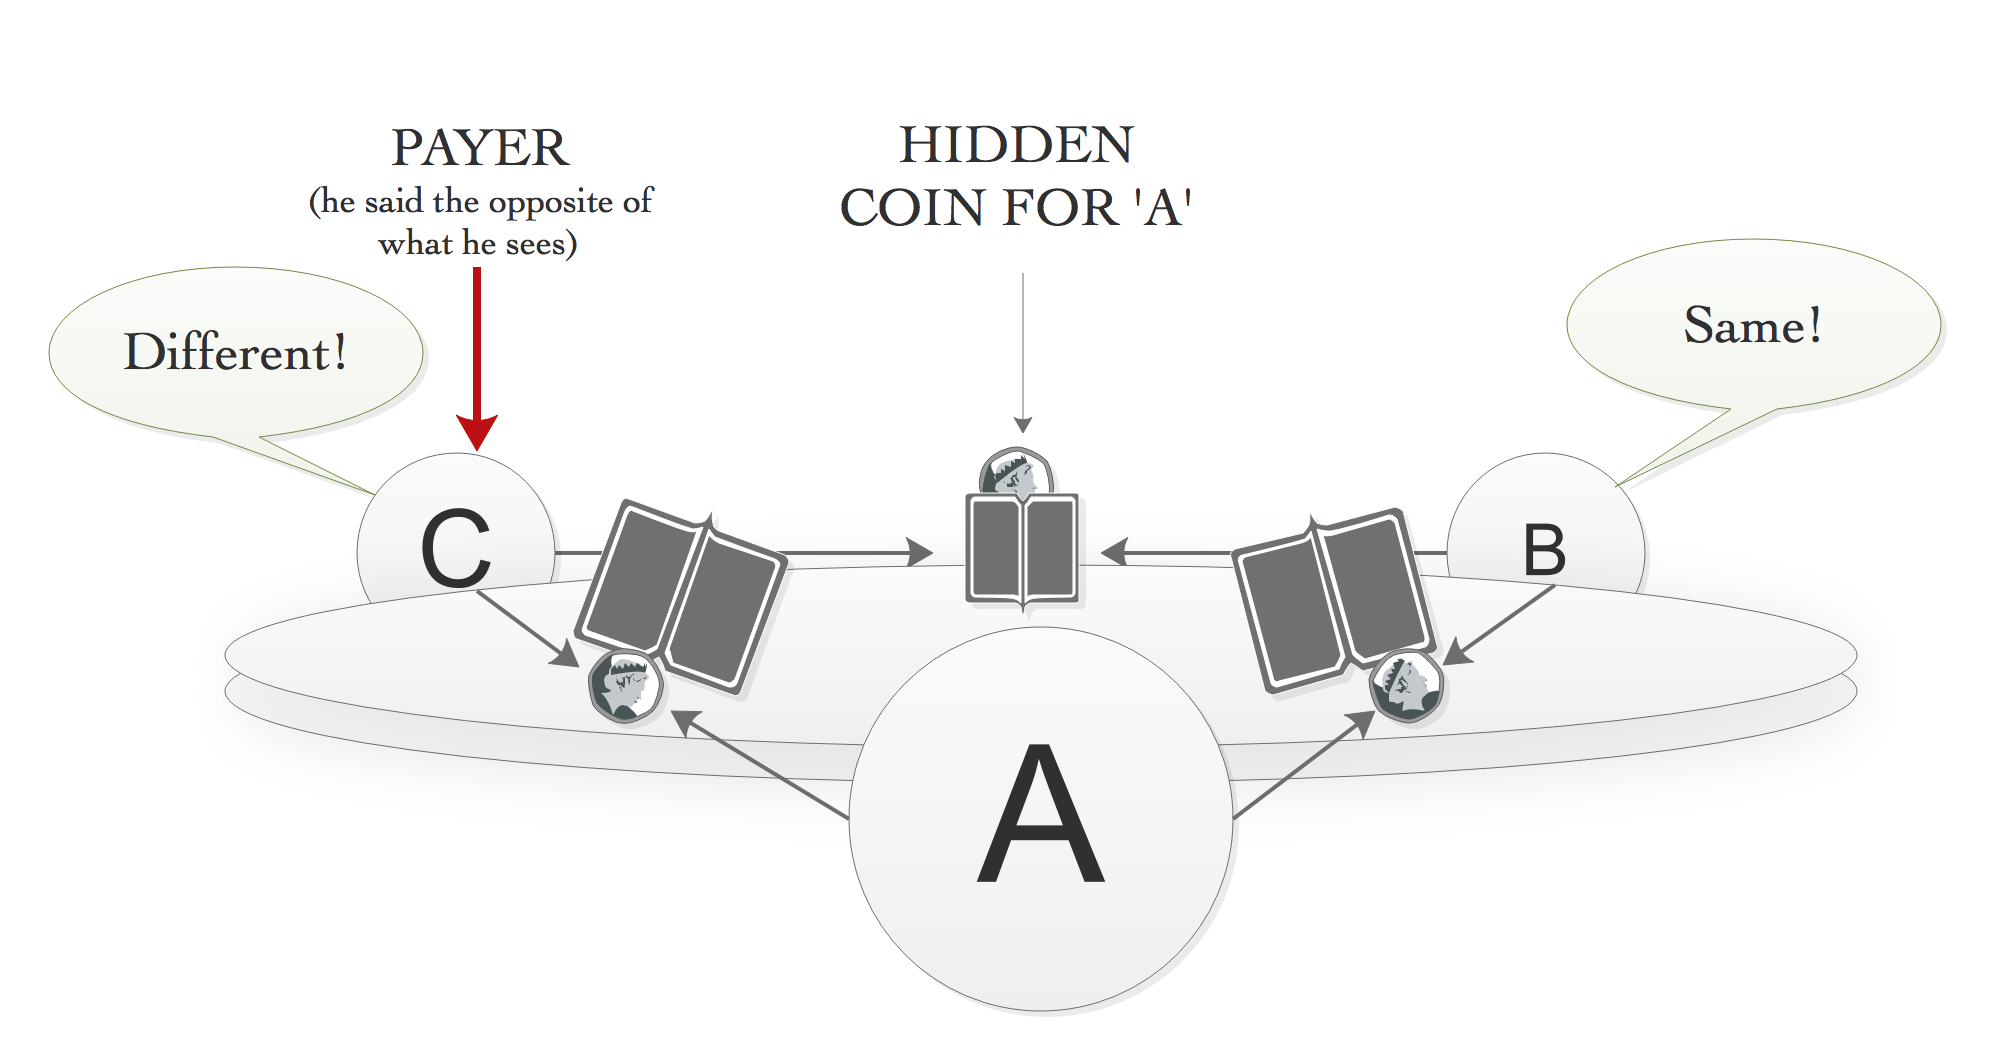
\includegraphics[width=0.80\textwidth]{Images/AsameCase1.png}
            \caption{Hidden Coin same as what A sees. C is the Payer.}
            \label{fig:AsameCaseSame}
        \end{figure}
        \begin{figure}[h!]
            \centering
            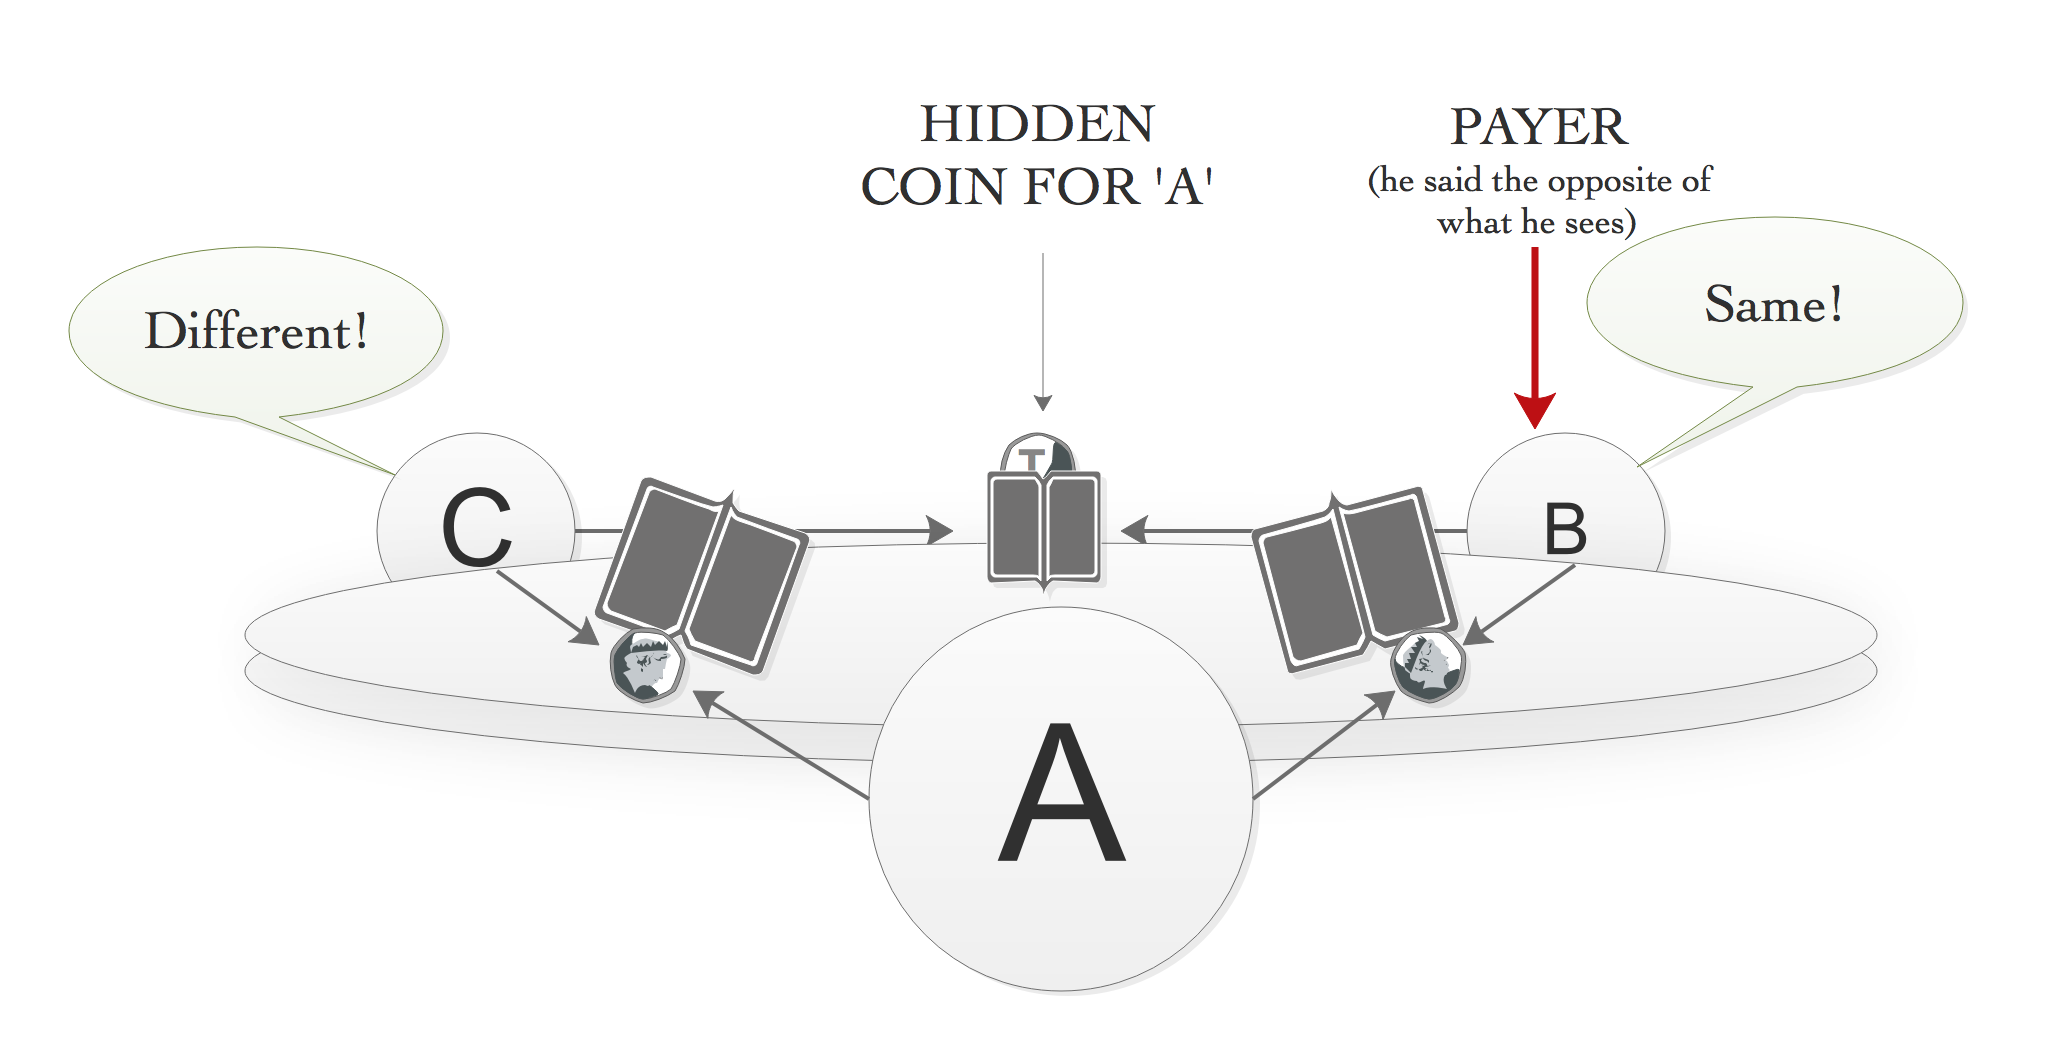
\includegraphics[width=0.80\textwidth]{Images/AsameCase2.png}
            \caption{Hidden Coin different from what A sees. B is the Payer.}
            \label{fig:AsameCaseDifferent}
        \end{figure}
        \item subject A sees two different coins (1 head and 1 tail). Then, if both the other cryptographers say 'Different', the payer is the one closest to the coin that A sees that is the same as the hidden coin (Figure \ref{fig:AdifferentCaseDifferent}); if both cryptographers say 'Same', the payer is the one closest to the coin that A sees that is different from the hidden coin (Figure \ref{fig:AdifferentCaseSame}) \cite{Chaum};
        \begin{figure}[h!]
            \centering
            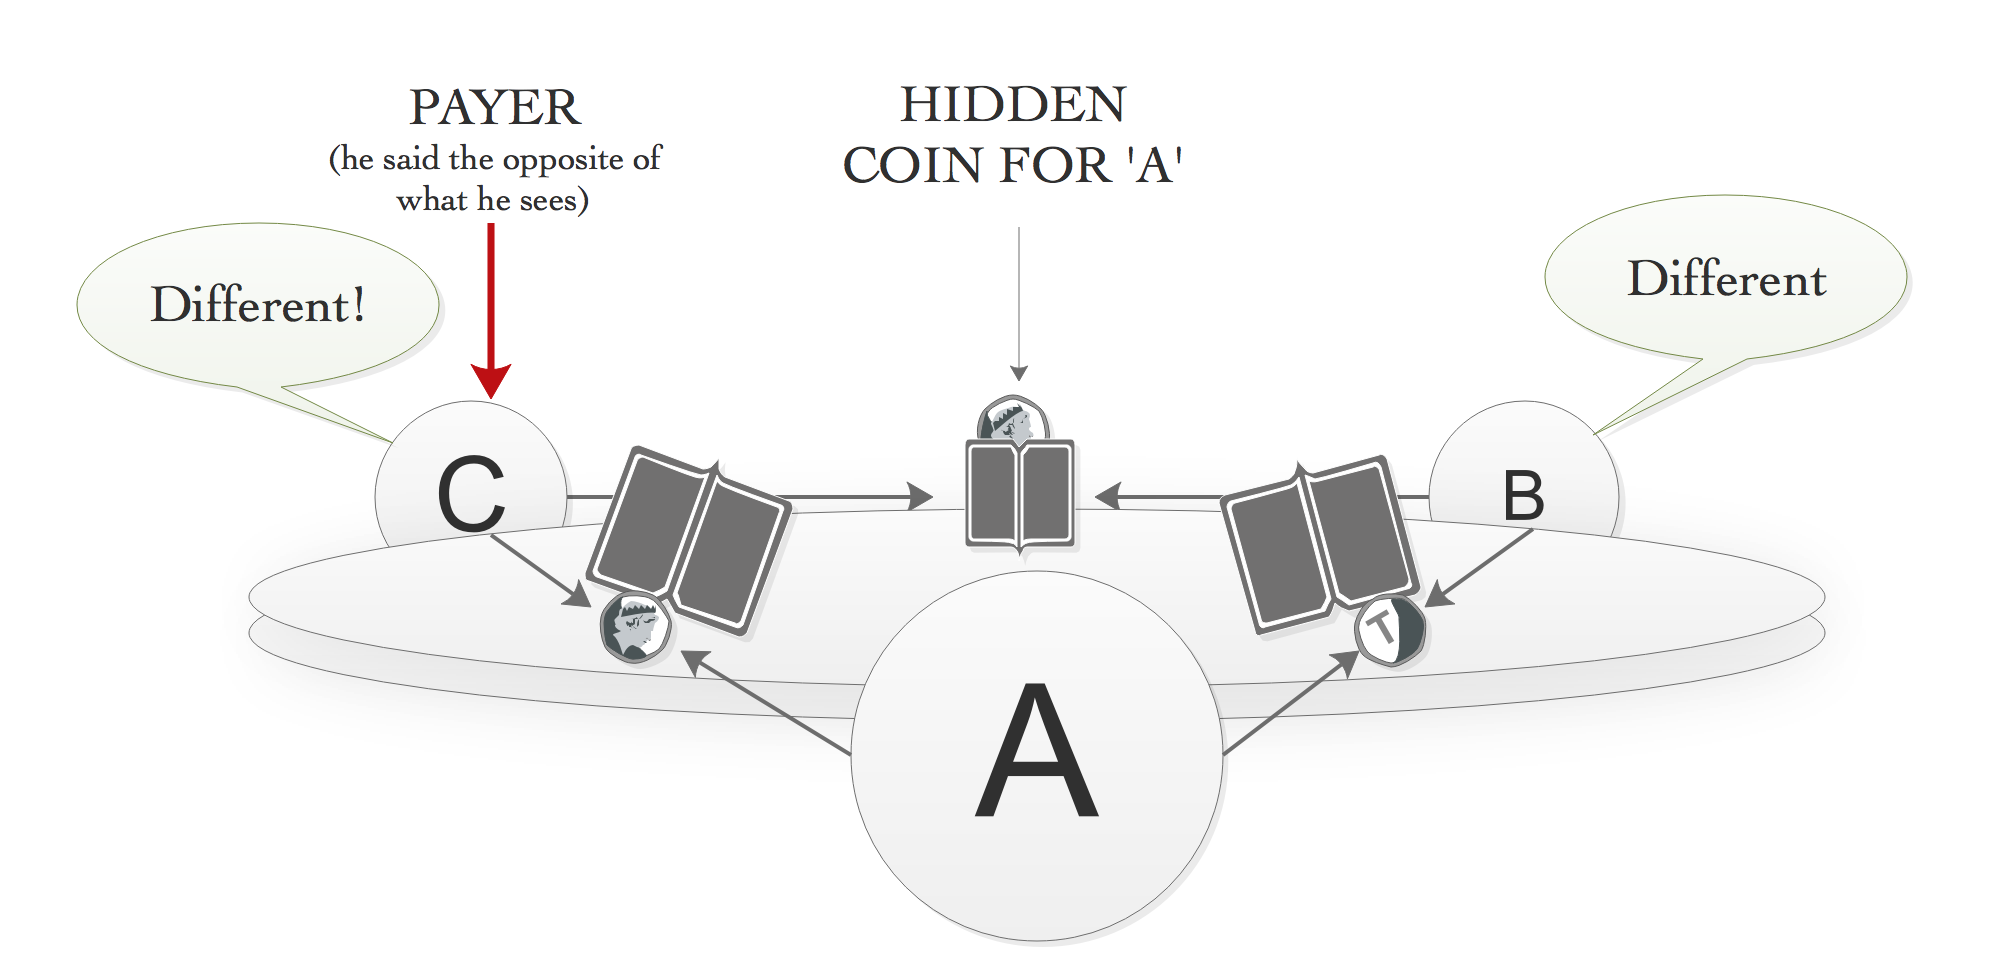
\includegraphics[width=0.80\textwidth]{Images/AdifferentCaseDifferent.png}
            \caption{Both Cryptographers say 'Different'. C is Payer.}
            \label{fig:AdifferentCaseDifferent}
        \end{figure}
        \begin{figure}[h!]
            \centering
            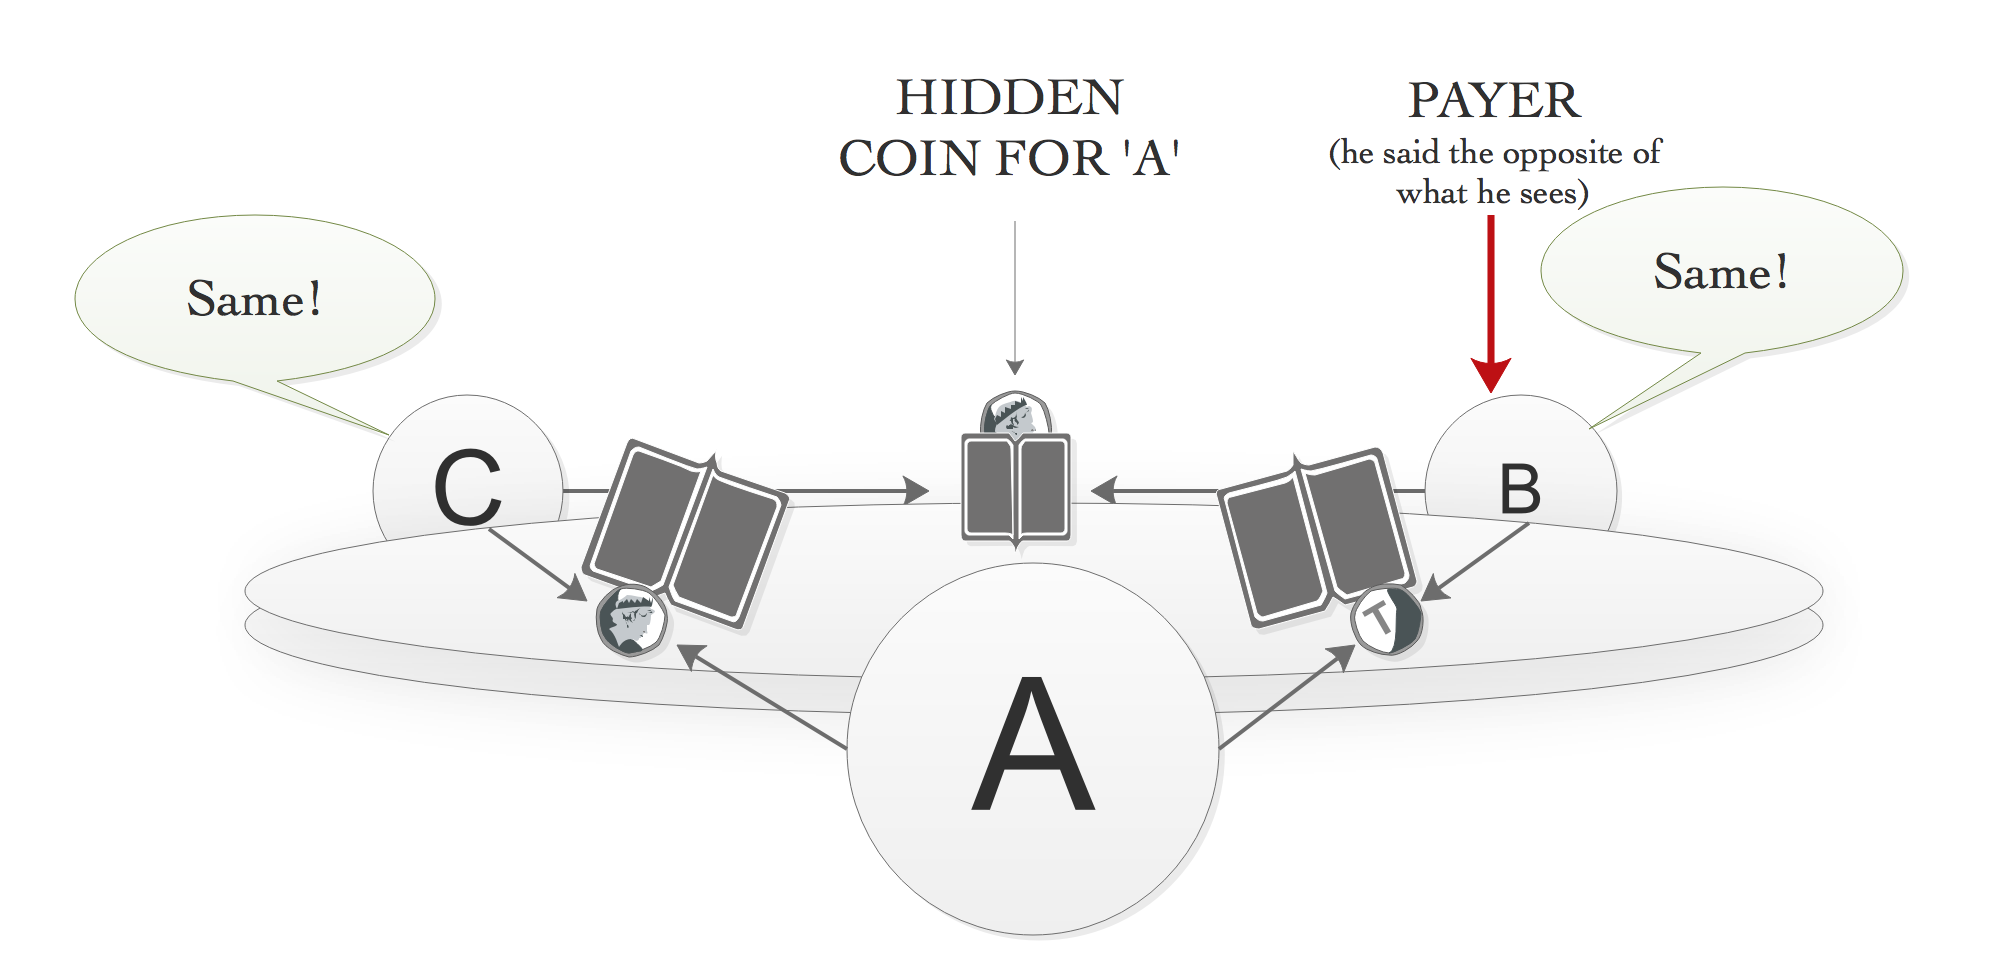
\includegraphics[width=0.80\textwidth]{Images/AdifferentCaseSame.png}
            \caption{Both Cryptographers say 'Same'. B is the Payer.}
            \label{fig:AdifferentCaseSame}
        \end{figure}
    \end{enumerate}
\end{enumerate}


As demonstrated in the scenarios above, the minimum number of participants required to carry out this protocol is three. If only two participants were present, sender anonymity would be guaranteed only in respect to an external observer of the network but not internally. Moreover, since the coin is unbiased, both head or tail have a 50{\%} likelihood of being the result. With such probability, a non-payer cryptographer can only guess the outcome of the hidden coin. Therefore, Chaum's protocol is unconditionally secure. \label{sec:internalExternalAnon}



\subsection{A Formal Exposition of the Protocol}
The analogy above has the purpose of facilitating the more formal exposition of the DC-Net protocol, which we present below. 

The Dining Cryptographers can be represented in graph theory, where each cryptographer is shown as a vertex. The flip coin presented in the analogy corresponds to a key exchange in a formal protocol. This key exchange is represented as an edge between two vertices, i.e. cryptographers. 

The basic version of the protocol uses one-bit keys. Therefore, only two values are possible, since a single bit can either be a 1 or a 0. From the metaphor of the coin, the head corresponds to a 1 and a tail is a 0 or vice versa.
The action of 'paying the dinner' corresponds to a participant, ergo a vertex, reversing his outcome before the broadcast. The action of 'announcing the result out loud' is a message broadcasted in the network. Lastly, each anonymous dinner payment is equivalent to a round of communication in which a node may broadcast a message.

\subsubsection{Exclusive OR (XOR)}
The operations executed by each cryptographer in stage 2 (see section \ref{sec:protocolStages}) to combine the results of different key-exchanges is done through the utilization of a logic operation called \textit{exclusive disjunction} or \textit{XOR}. The logical operation outputs true only if the the input values are different (table \ref{table:XOR}). The symbol of this operation is "$\oplus$".

\begin{table}[h!]
\centering
\caption{XOR Truth Table}
~\\[0.5ex]
\begin{tabular}{|| c | c | c ||} 
 \hline
 X & Y &  $X \oplus Y$ \\ [0.ex] 
 \hline\hline
 0 & 0 & 0 \\ 
 0 & 1 & 1 \\
 1 & 0 & 1 \\
 1 & 1 & 0 \\ [1ex]
 \hline
\end{tabular}
\label{table:XOR}
\end{table}

The XOR operation is also executed to combine the result of each vertex, i.e. cryptographer, at the third stage of the protocol, where at least three bits are present - one for each cryptographer in the network (see section \ref{sec:protocolStages}). In this case, the overall operation can be seen as a cascade of XOR operations between two input at a time (table \ref{table:XORextended}).


\begin{table}[h!]
\centering
\caption{XOR Truth Table with multiple values}
~\\[0.5ex]
\begin{tabular}{|| c | c | c | c ||} 
 \hline
 X & Y & Z & $(X \oplus Y) \oplus Z$ \\ [0.ex] 
 \hline\hline
 0 & 0 & 0 & 0 \\ 
 0 & 0 & 1 & 1 \\
 0 & 1 & 0 & 1 \\
 0 & 1 & 1 & 0 \\
 1 & 0 & 0 & 1 \\
 1 & 0 & 1 & 0 \\
 1 & 1 & 0 & 0 \\ 
 1 & 1 & 1 & 1 \\ [1ex]
 \hline
\end{tabular}
\label{table:XORextended}
\end{table}

The mathematical properties of the XOR operation are also very relevant for DC-Net problem \cite{Lewin} and are four:
\begin{enumerate} \label{sec:XORproperties} \label{sec:xorproperties}
    \item \textit{Commutative:} It does not matter the order of the inputs. $A \oplus B = B \oplus A$
    \item \textit{Associative:} XOR operation can be chained in any order $A \oplus (B \oplus C) = (A \oplus B) \oplus C$
    \item \textit{Identity Element:} XORing a value with zero will not change the value. $A \oplus 0 = A$
    \item \textit{Self-Inverse:} Any value XOR'd twice will cancel itself. In other words, a value XOR's with itself is equal zero. $A \oplus A = 0$
\end{enumerate}

\subsubsection{Exchange of one-bit messages with \textit{3} participants}
The following is the scenario and procedure of the protocol executed with the minimum number of three participants and expressed with a more formal notation (examples in figure \ref{fig:dcFormalnoMessage} and \ref{fig:dcFormalWithMessage}) :
\begin{enumerate}
    \item There are 3 vertices \textit{$P_1, P_2, P_3$};
    \item Each vertex is part of two adjacencies, one for each neighbour. For example, vertex \textit{$P_1$} is part belongs to \textit{$N(P_1,P_2)$} and \textit{$N(P_1, P_3)$};
    \item Each adjacency is also an edge that represents a key. \textit{$P_1$} will have edges \textit{$K_{1,2}$} and \textit{$K_{1,3}$};
    \item Each vertex will calculate the value to be broadcasted. In the example of \textit{$P_1$}: 
    \begin{enumerate}
        \item If P1 does not want to send a message ($M_1$), \textit{$M_1 = K_{1,2} \oplus K_{1,3} \oplus 0 $}. This is equivalent to \textit{$M_1 = K_{1,2} \oplus K_{1,3}$};
        \item If P1 wants to send a message ($M_1$) \textit{$M_1 = K_{1,2} \oplus K_{1,3} \oplus 1 $}. This is equivalent to \textit{$M_1 = \neg(K_{1,2} \oplus K_{1,3}) $};
    \end{enumerate}
    \item The final round result (R) will be calculated by XORing all the results such that \textit{$R = M_1 \oplus M_2 \oplus M_3$}.
\end{enumerate}


\begin{figure}[h!]
    \centering
    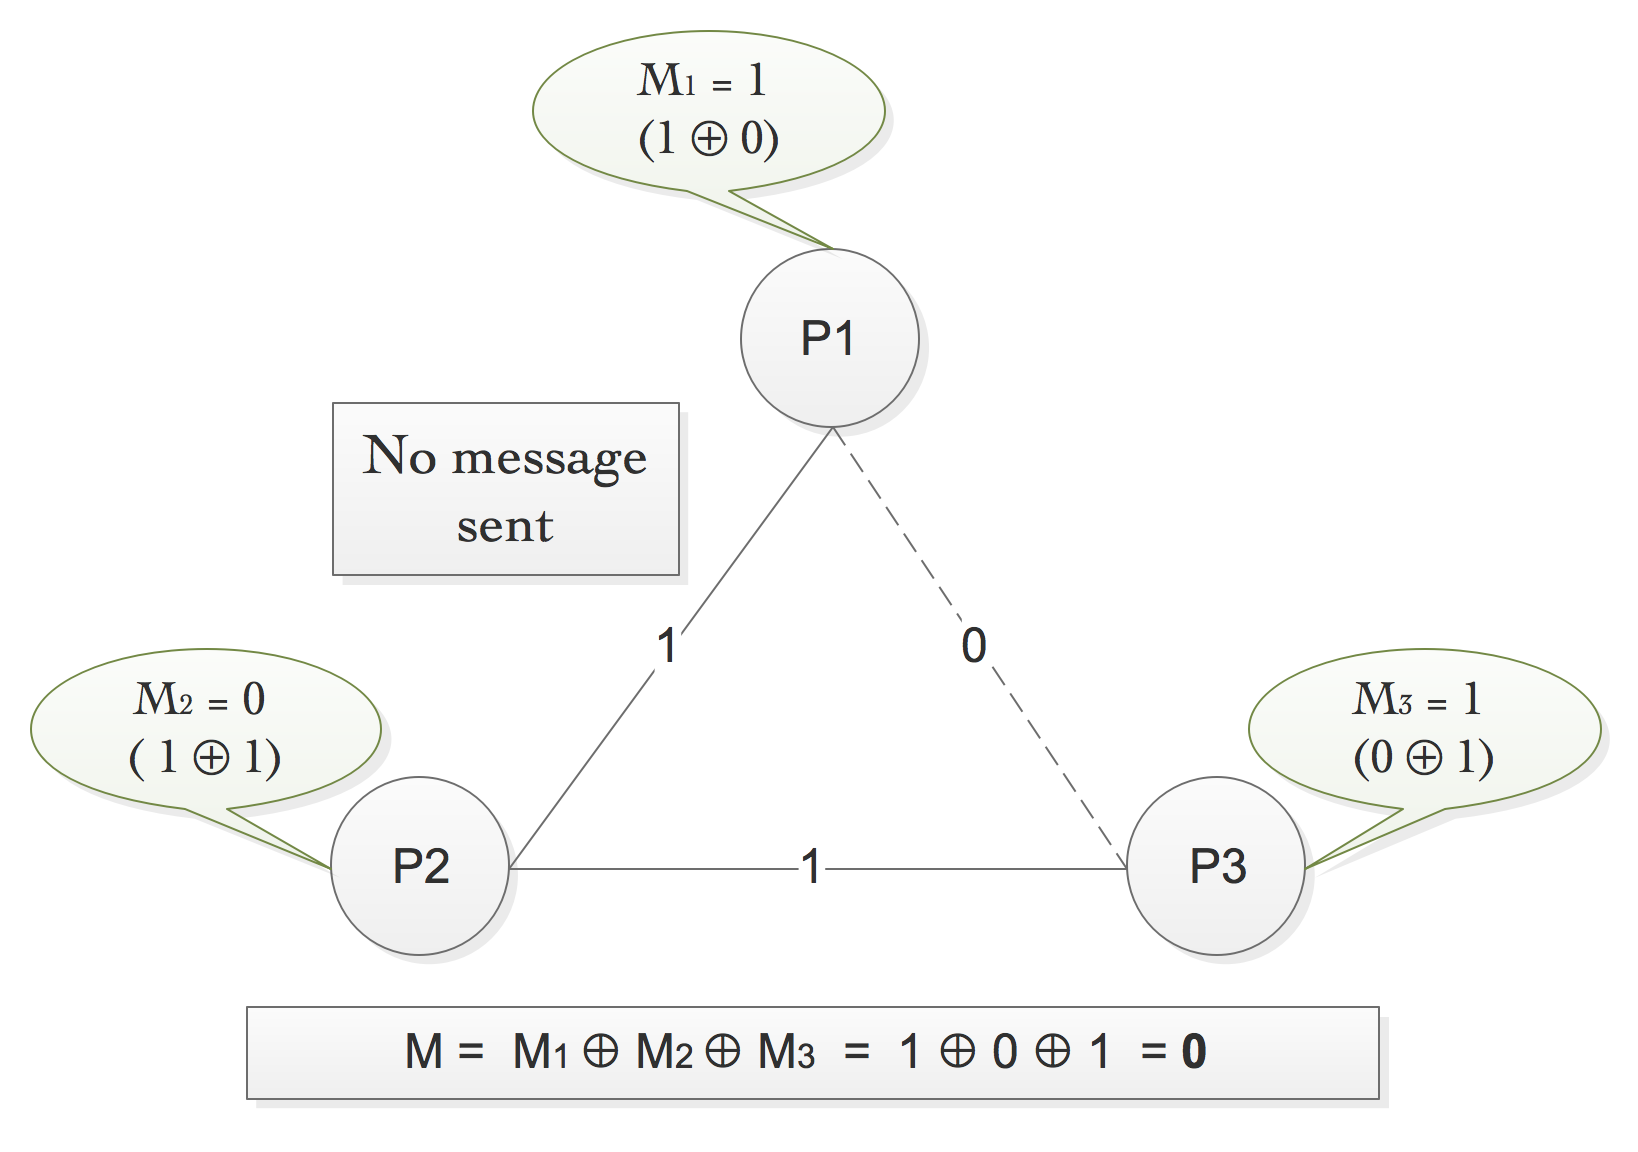
\includegraphics[width=0.70\textwidth]{Images/DCFormalNoMessage.png}
    \caption{3 vertices message exchange with no message sent (even number of 1s)}
    \label{fig:dcFormalnoMessage}
\end{figure}

\begin{figure}[h!]
    \centering
    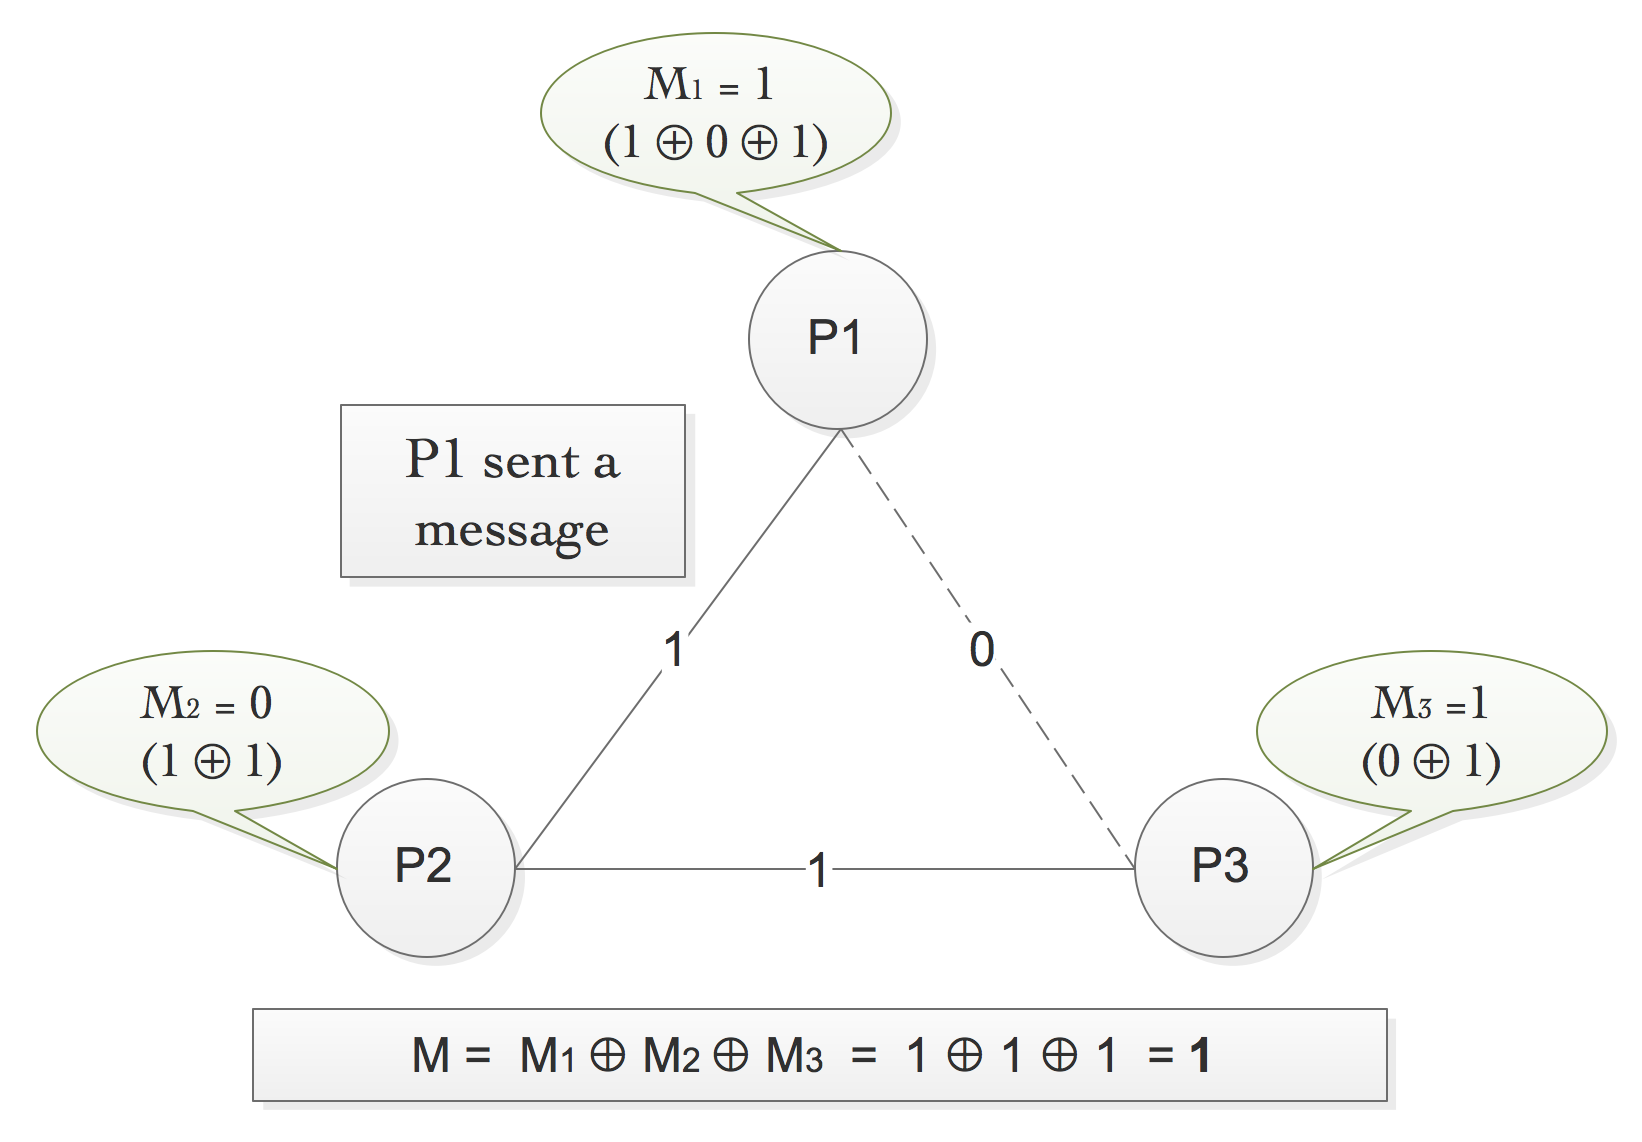
\includegraphics[width=0.70\textwidth]{Images/DCFormalWithMessage.png}
    \caption{3 vertices message exchange with a message sender (odd number of 1s)}
    \label{fig:dcFormalWithMessage}
\end{figure}

From now on, the dinner analogy language and the formal graph notation will be used interchangeably. \newline \newline \newline

\section{Limitations}
As already mentioned, the Dining Cryptographer is a very effective protocol to guarantee sender anonymity in \textit{theory}. In reality, there are some limitations, which affect the practicality of the protocol in a real-world use to the point there does not exist a fully-working version of this protocol.
The three main limitations we now turn to explore are: message collision, communication disruption and communication overhead. 

\subsection{Collisions}
A message collision is the attempt of two cryptographers to send a message in the same round of communication.So far, one of the assumptions to verify the correctness and efficacy of the protocol was that only one vertex, or cryptographer, broadcasts a message per round. However, it is possible and likely that multiple vertices will try to send a message, i.e. a reversed response, in the same round, which leads to a message collision. The consequence is that, if an even number cryptographers sends a message in the same round, the final result will be 0, which equates to 'no one has flipped their message'. If an odd number of cryptographers sends a message in the same round, the final result will be 1, which corresponds to just one cryptographer having sent a message.
Therefore, if this probable scenario is not acknowledged, the correctness of the protocol is jeopardized.

\subsection{Disruption and Collusion} \label{sec:disruptionlimitation}
Disruption and collusion are two limitations brought by the presence of active attackers in the network. A passive attacker is a principal that can only intercepts messages being exchanged, eavesdropper. An active attacker, on the other hand, performs malicious actions, such changing the content of a messages before sending it. The protocol is secure in respect to an eavesdropper. However, a cryptographer inside the network, who is an active attacker, could inject falsified responses instead of following the protocol rules. Unless these forged messages are somehow detected, this can easily disrupt the execution of the protocol.

Another possible problem may be incurred by an active attacker delaying his responses at each round. Since the final result of the round cannot be calculated unless all the clients have provided their responses, such delay may affect the availability of the service \cite{Fischer}.

Moreover, active attackers within the network may collaborate to uncover the real sender of a message by pooling together their keys. This possible threat is called collusion. Assuming three participants in the network and one cryptographer discovering the value of the third hidden coin via key pooling with one of his neighbours, this malicious cryptographer can establish who sender is, if any is present \cite{Chaum}. 

This type of collaboration is treated in more depth by other information security academics, such as Waidner \cite{Waidner} or Safavi-Naini and Susilo \cite{Susilo}. As established by several academic analyses, the technical capability of colluding also depends on the key-sharing topology implemented, therefore this limitation may be mitigated by using specific architectures (see section \ref{sec:participantsextention}). 


\subsection{Communication Overhead} \label{sec:complexitylimitation}
An overhead is an excess of computation power or resources needed to perform a specific task. 

Depending on the architecture implemented, there are several messages to be sent in order to hide the real sender. Each client is part of two messages per round of communication: one message sent as part of the sender anonymity set and one message is received as part of the recipient anonymity set.

In the key-sharing graph explained so far (see section \ref{sec:ringtopology}), given $n$ participants, a single bit message will require at least $2n$ messages to be sent on the network in a single round. 

In another architecture presented later in section \ref{sec:fullmeshtopology}, each client broadcasts $n-1$ messages, leading to $2(n * (n - 1))$ exchanges per round.

This overhead is necessary to guarantee anonymity and the larger the $n$ the higher the level of anonymity, as seen in section \ref{sec:anonymityset}. 

The operating cost is likely to be the main reasons why such powerful protocol is deemed impractical \cite{Scholz}.


\section{Extensions of Basic Protocol}

The basic protocol is presented with specific message length (one-bit messages) and a given number of participants (three). However, in the real world, it is highly unlikely that a network would exhibit three participants exchanging only one-bit messages. Based on such features, the pertinence of the protocol is restricted to an unrealistic scenario. 

To extend the applicability of Chaum's protocol, we can consider more participants and more complex messages within the network as per below.

\subsection{Increase number of participants} \label{sec:participantsextention}
The basic protocol can be generalized to accommodate \textit{n} participants (more than 3) with two different topologies.

\subsubsection{Ring Topology} \label{sec:ringtopology}
One of the two methods to extend the protocol to multiple payers is very similar to the one presented up to this point. Each vertex will have only two edges, one with each neighbour, and the protocol follows the same rules, as showed in figure \ref{fig:nparticipants1}.

More formally speaking: 
\begin{enumerate}
    \item There are \textit{n} vertices named \textit{$P_1, P_2, ..., P_n$};
    \item Each vertex \textit{$P_i$} is part of two adjacencies, one for each neighbour: \textit{$N(P_i,P_{i-1}), N(P_i, P_{i+1})$};
    \item Each adjacency is also an edge that represents a key: \textit{$K_{i,i-1}$} and \textit{$K_{i,i+1}$};
    \item Each vertex will calculate the value to be broadcasted as follows: \begin{enumerate}
        \item If the node does not want to send a message \textit{$M_i = K_{i,i-1} \oplus K_{i,i+1} \oplus 0 $}. This is equivalent to \textit{$M = K_{i,i-1} \oplus K_{i,i+1}$};
        \item If the node wants to send a message \textit{$M_i = K_{i,i-1} \oplus K_{i,i+1} \oplus 1 $}. This is equivalent to \textit{$M_i = \neg(K_{i,i-1} \oplus K_{i,i+1}) $};
    \end{enumerate}
    \item The final round result will be calculated by XORing all the results such that \textit{$R = M_1 \oplus M_2 \oplus ... \oplus M_n$} (example in figure \ref{fig:nparticipants1}).
\end{enumerate}


\begin{figure}[h!]
    \centering
    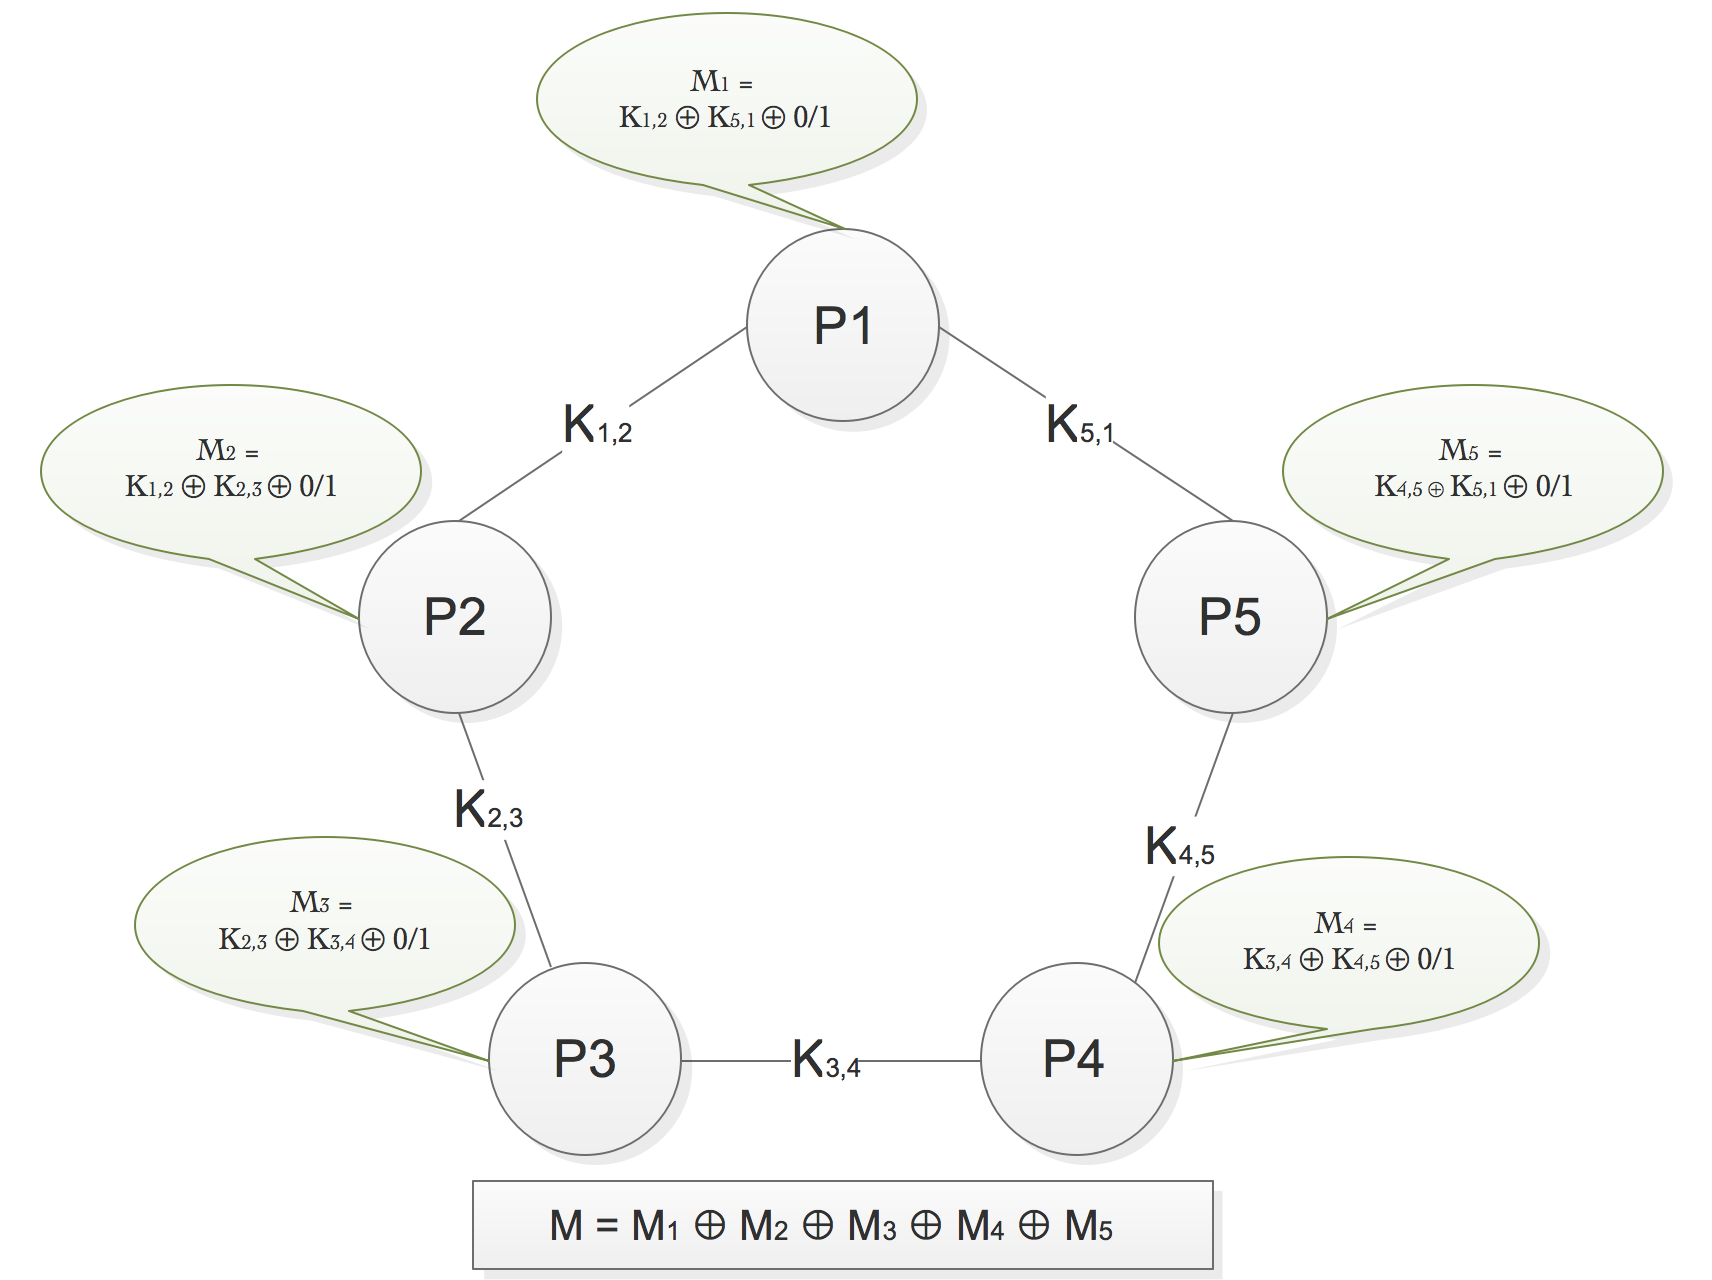
\includegraphics[width=0.95\textwidth]{Images/nparticipants1.png}
    \caption{Message exchange of 5 participants with ring topology}
    \label{fig:nparticipants1}
\end{figure}


\subsubsection{Full Mesh Topology} \label{sec:fullmeshtopology}
The second approach, presented by Chaum, differs in the respect that each vertex has an edge connecting with every other vertex \cite{Chaum}. Therefore, whichever pair of cryptographers, no matter if they are adjacent or not, shares a secret key. In such scenario, each vertex holds \textit{$n - 1$} keys, and his response will be the result of XORing all these values. The message a cryptographer sends is flipped, hence XORed with 1, if he  wishes to send a message.

More formally speaking:
\begin{enumerate}
    \item There are \textit{n} vertices named \textit{$P_1, P_2, ..., P_n$};
    \item Each vertex has \textit{$n-1$} edges that represent the same number of keys key: \textit{$K_{i,i-1}, K_{i,i+1}, ... , K_{i,n} $} (excluding \textit{$K_{i,i}$});
    \item Each vertex will calculate the value to be broadcasted \textit{$M_i = K_{i,i-1} \oplus K_{i,i+1} \oplus ... \oplus K_{P_i,P_n} $}. \textit{M} will be reversed if \textit{$P_i$} wants to broadcast his 1 bit message.
    \item The final round result will be calculated by XORing all the results such that \textit{$R = M_1 \oplus M_2 \oplus ... \oplus M_n$} (Example in figure \ref{fig:nparticipants2}). \newline
\end{enumerate}


\begin{figure}[h!]
    \centering
    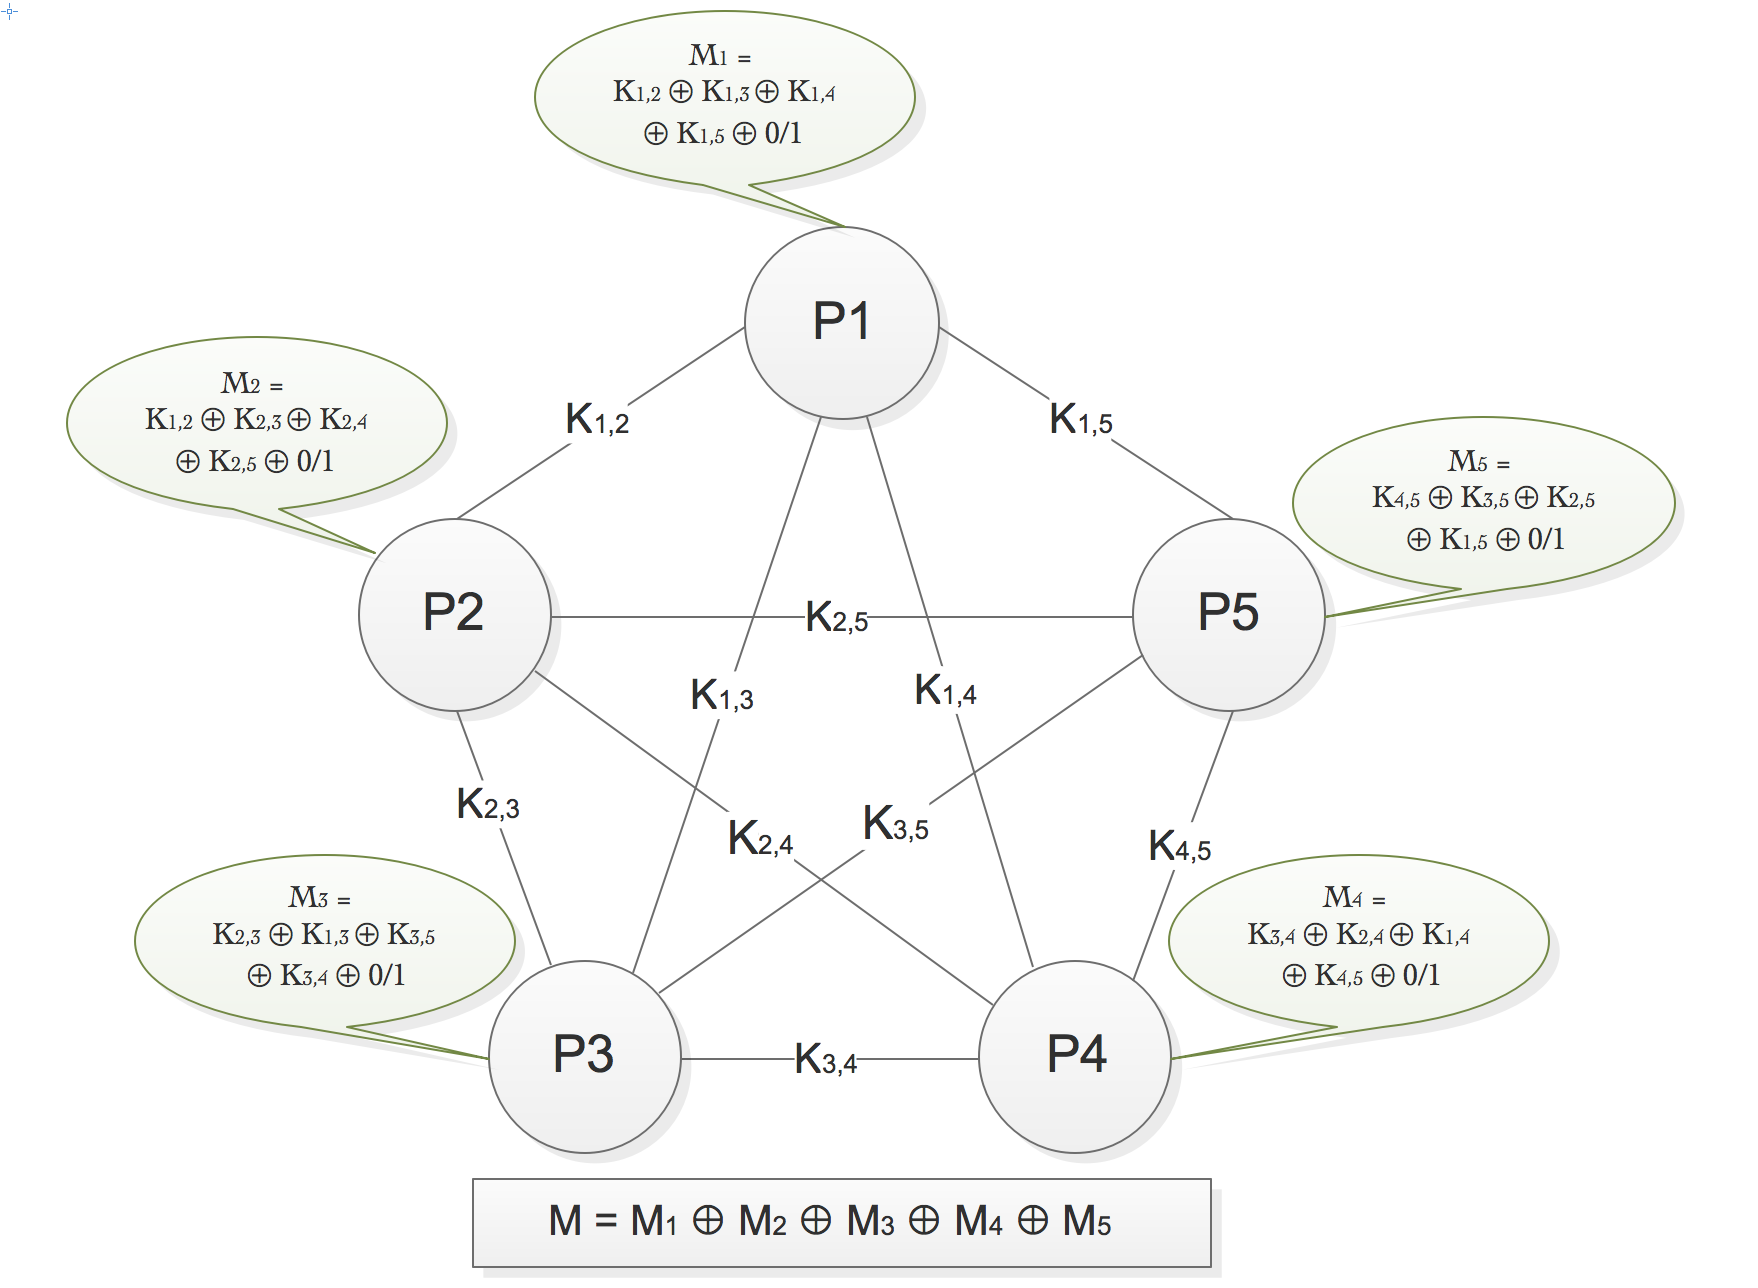
\includegraphics[width=0.95\textwidth]{Images/nparticipants2.png}
    \caption{Message exchange of 5 participants with full-mesh topology}
    \label{fig:nparticipants2}
\end{figure}


Each approach presents advantages over the other. A ring topology uses less computational power therefore presents less overhead, as explained in section \ref{sec:complexitylimitation}, while a full-mesh topology can be considered more secure against collusion of participants, explained in section \ref{sec:disruptionlimitation}.
The overall benefit of multiple participants within a network is twofold:
\begin{enumerate}
    \item adapting the protocol to a real-world scenario as it is unreasonable to have a network with only three nodes;
    \item growing the number of participants increases the level on anonymity as explained in section \ref{sec:anonymityset}; \newline \newline
\end{enumerate} 

\subsection{Extend message length}

Accommodating many participants makes the protocol more suitable for a real application. So does the possibility of sending longer messages. Increasing the length of messages to more than one bit may have two possible meanings: (1) to send different keys that are longer than one bit or (2) to repeat the round multiple times in order to gather pieces of the same message.

\subsubsection{Keys longer than one bit} \label{sec:longerKeys}
The range of possible keys can be incremented by growing the number of bits in a key. If the keys are, for example, 8-bit long, the possible randomly generated value of a key can be anything between 0 and 255 ($2^8$), as opposed to a 1-bit key where values can only be 0 or 1 ($2^1$) \cite{Scholz}. A 1-bit key network allows a sender cryptographer to XOR his two secret keys with a 0 or 1, which corresponds to flipping a message (see section \ref{}). A 8-bit key network allows the sender cryptographer to XOR his two secret keys with a value, i.e. anonymous message, that can be anything between 0-255 as the range of the key. An example is provided in figure \ref{fig:xorlongkeys}.

\begin{figure}[h!]
    \centering
    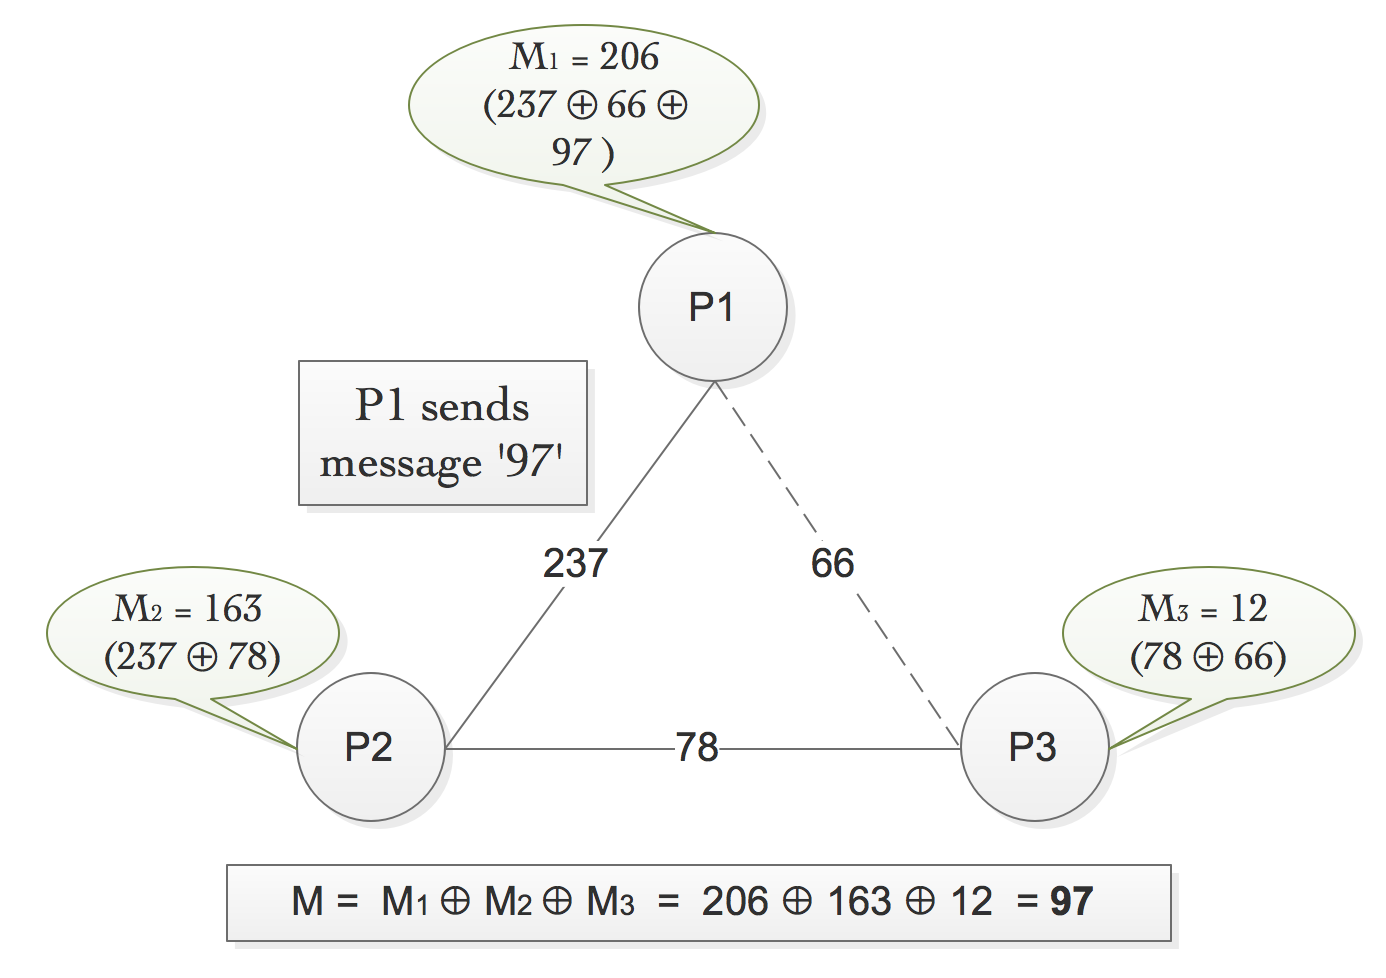
\includegraphics[width=0.95\textwidth]{Images/dcnet8bitkeys.png}
    \caption{Three participants round with 8-bit keys}
    \label{fig:xorlongkeys}
\end{figure}

Adopting longer keys can be useful. Take, for example, the ASCII character encoding, a technique to represent a character (e.g. a number, symbols or letters) has a corresponding number. The official ASCII encoding contains 128 characters, and the extended version has 256 of them, which can therefore represented in 8 bits ($2^8$). Therefore, a cryptographer wanting to send a specific letter may simply XOR his two secret keys with the ASCII number that represents the said letter.


\subsubsection{Multiple Rounds} \label{sec:messageExtentionRounds}
An alternative to sending longer messages is to repeat the protocol multiple times. The repetition allows a node to send multiple messages in a row, either with a 1-bit key or in conjunction with the long-key technique explained in the previous section. By repeating the protocol multiple rounds, a cryptographer can broadcast a cumulative message that might be more meaningful that a single round of communication.



\section{Practical Considerations}
As we have discussed, the Dining Cryptographers protocol tries to jointly compute the result of a function from different nodes. Such type of protocol is a specific sub-field of cryptography called 'secure multi-party computation' \cite{wiki1}. 

The fact that nodes do not reside in the same physical location, adds further complications to the scenario, such as the network topology used to implement the protocol, the implications of the distributed architecture over the protocol's computation and the method of transmission of the secret one-time keys  to each node.

(What network topology is it used to implement this protocol? 

What implication has the distributed architecture over the protocol computation? 

As DC-Net relies on confidential one-time keys, how does such secret reach each node?)

\noindent \newline These practical issues are addressed in this section to start considering what are the repercussions of implementing a protocol that, in theory, provides flawless sender anonymity.


\subsection{Key Exchange Channels} \label{sec:keyExchangeMethods}
A fundamental problem in cryptography to ensure the effectiveness of a protocol is how to exchange keys securely. The DC-net is no exception: in order to guarantee the anonymity of the senders and recipient in the network, the single part of communication that needs to be securely completed is the exchange of the keys.

\subsubsection{Physical Disks}
In its original paper, Chaum proposes the exchange of physical optical disks that with today's storage capabilities can provide trillions of randomly-generated bits to be used as keys \cite{Chaum}. However, this is impractical for real-world applications, especially for large networks. 

\subsubsection{Synchronised Number Generators}
Another possibility is to use synchronised cryptographically secure pseudo-random number generators (CSPRNG). This entails that each client has its own generator and no key is ever transmitted on the network. Consequently, the reliability of the DC-net protocol would be based on the implementation of the generators \cite{Chaum}.

\subsubsection{Public-key Cryptography}
Lastly, a practical alternative is to use public-key cryptography. The most commonly used methods are \cite{Chaum}:
\begin{enumerate}
    \item RSA cryptosystem: employing a pair of private and public key for each client in order to encrypt keys securely;
    \item Diffie-Hellman 'key-exchange': a key generation protocol that can work on completely insecure communication channels to create keys for participants without ever transmitting it over the network \cite{Golle}.
\end{enumerate}


\subsection{Possible Network Topologies} \label{sec:networkTopologies}
There are two main network topologies that can be used in order to implement a DC-Net: peer-to-peer an client-server. The network topology is not to be confused with the key-exchange topologies presented in section \ref{sec:participantsextention}.

\subsubsection{Peer-to-Peer} \label{sec:peertopeer}
This topology resembles closely the description of the protocol so far, in which a node communicates directly with his neighbours or with all participants in the network. This setting requires nodes to handle the whole of the communication, key generation, and broadcast.
Peer-to-peer does not provide a mechanism to detect collisions efficiently, since each nodes cannot know if neighbours are sending their correct responses or if they are adding a message to their broadcast.


\subsubsection{Client-Server} \label{sec:clientserver}
A client-server topology decreases the responsibilities of a node given the presence of a centralized DC-net service. Plus, the server has a much more complete vision of the network in respect to a node. \emph{This is a very contradictory factor}. On one hand, it offers the DC-Net various capabilities such as detecting collisions efficiently, generating keys, helping the clients broadcast messages at the same time. On the other hand, it introduces issue of \emph{trust}. The clients are supposed to believe that the server is a non-malicious entity that will facilitate the communication. In addition, if someone has access to the server and this is the place where the keys are generated, the protocol would be completely compromised.

\subsection{Detecting Collisions}
The protocol's limitation of potential collisions is to be addressed in order to transmit useful messages. Without such feature the protocol would be secure but useless. \newline

A DC-Net implementation that does not possess a DC-net central entity to coordinate the network, the collisions would be detected only by the actual message senders. For example, in a one-bit key message exchange, if a node transmits a message and the final broadcast results in no one having sent a message, then the node can deduct the presence of an even number of message senders in this given round. To tackle this issue, the said node can retransmit after a random number of communications rounds. \newline

The above collision-detection technique is not effective in a scenario in which a node would like to send a long message across multiple rounds (section \ref{sec:messageExtentionRounds}). This instance demands for an uninterrupted flow of communication without collisions, otherwise the meaning of whole message can be considered affected.
In this scenario, the only possible solution is to employee a server as central DC-Net service. This entity would be aware of who the message sender is so as to reserve a number of rounds only for that given node.


\section{Existing DC-net simulation tools} \label{sec:similarWorks}
It is important to research the area of interest of a project in the early stages of development in order to analyse the existing works, draw inspiration, and determine possible areas of improvement. \newline

The main purpose of this project is to develop a simulation tool for the Dining Cryptographers protocol. The outcome of the research of existing tools is in fact the leading motivation for implementing a DC-Net simulator. Namely, there is an easily identifiable gap in the domain of practical software systems that exemplifies the functioning of this protocol, whereas there is a wealth of academic papers that thoroughly examines the protocol on a theoretical level. 

In addition, the handful of projects found is of little help in deepening the understanding of the protocol since they are mostly command-line tools that, beside the unhelpful user experience in terms of graphics, are not well-documented on how to perform even a single round of communication. \newline

DC-Net is is mostly a theoretical concept, therefore researches on the wide internet lead exclusively to academic papers. A sensible approach to find possible implementations is to search through the development platform GitHub. Below are some implementation found, which highlight the shortcomings of the current state of art in DC-Net implementations.

\subsection{Example 1}
The first is a command line tool that presents extensive documentation, which appears to be very handy (figure \ref{fig:work1documentation}). However, all the commands listed in the documentation do not work, return errors, and there is no troubleshooting guide (figure \ref{fig:work1error}).

\begin{figure}[h!]
    \centering
    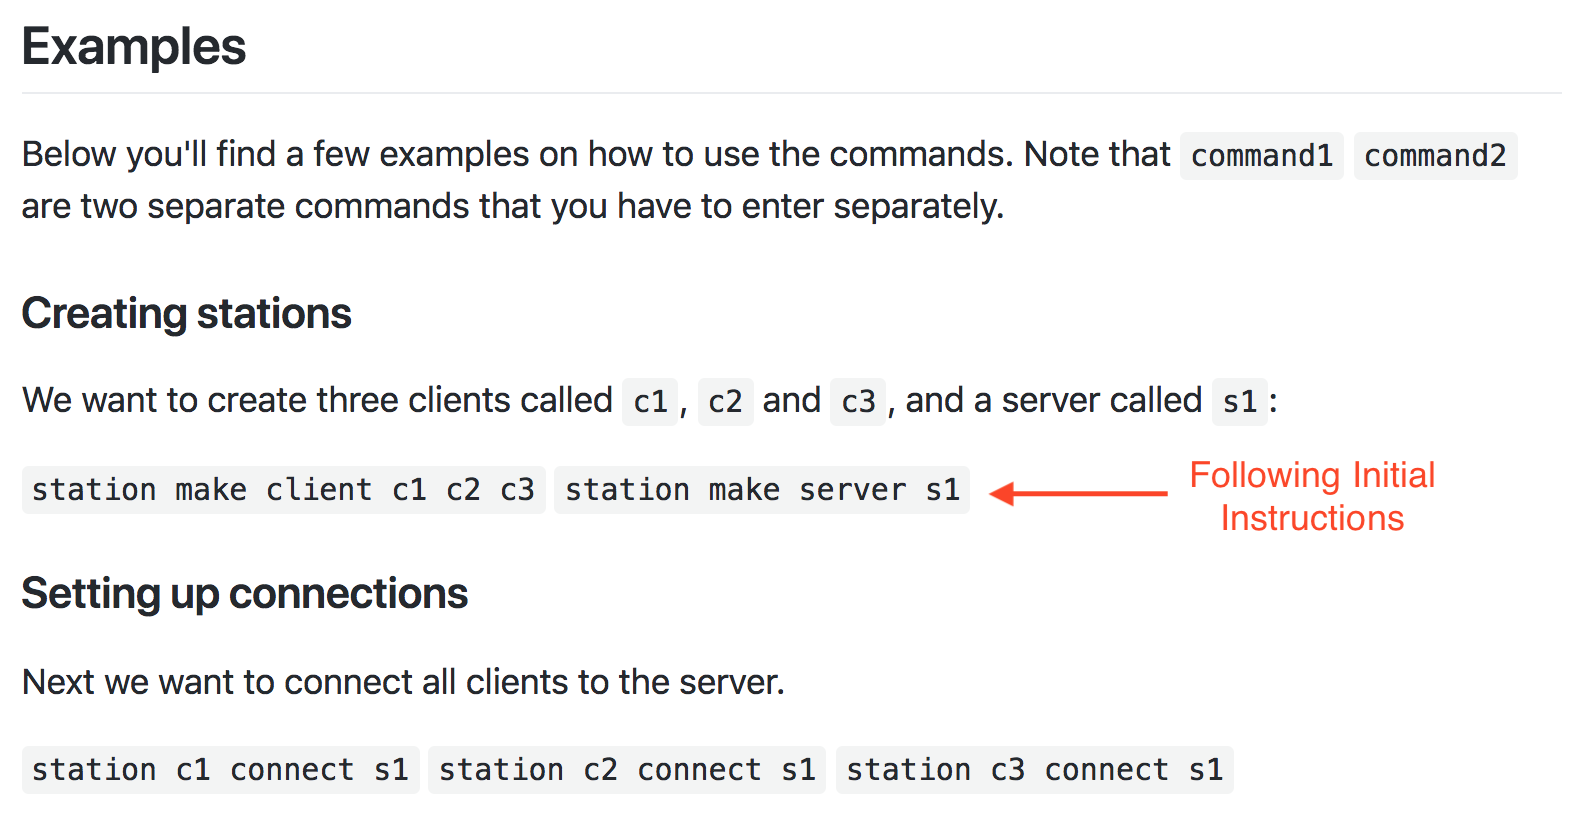
\includegraphics[width=0.7\textwidth]{Images/work1WellDocumented.png}
    \caption{Extensive encouraging documentation.}
    \label{fig:work1documentation}
\end{figure}

\begin{figure}[h!]
    \centering
    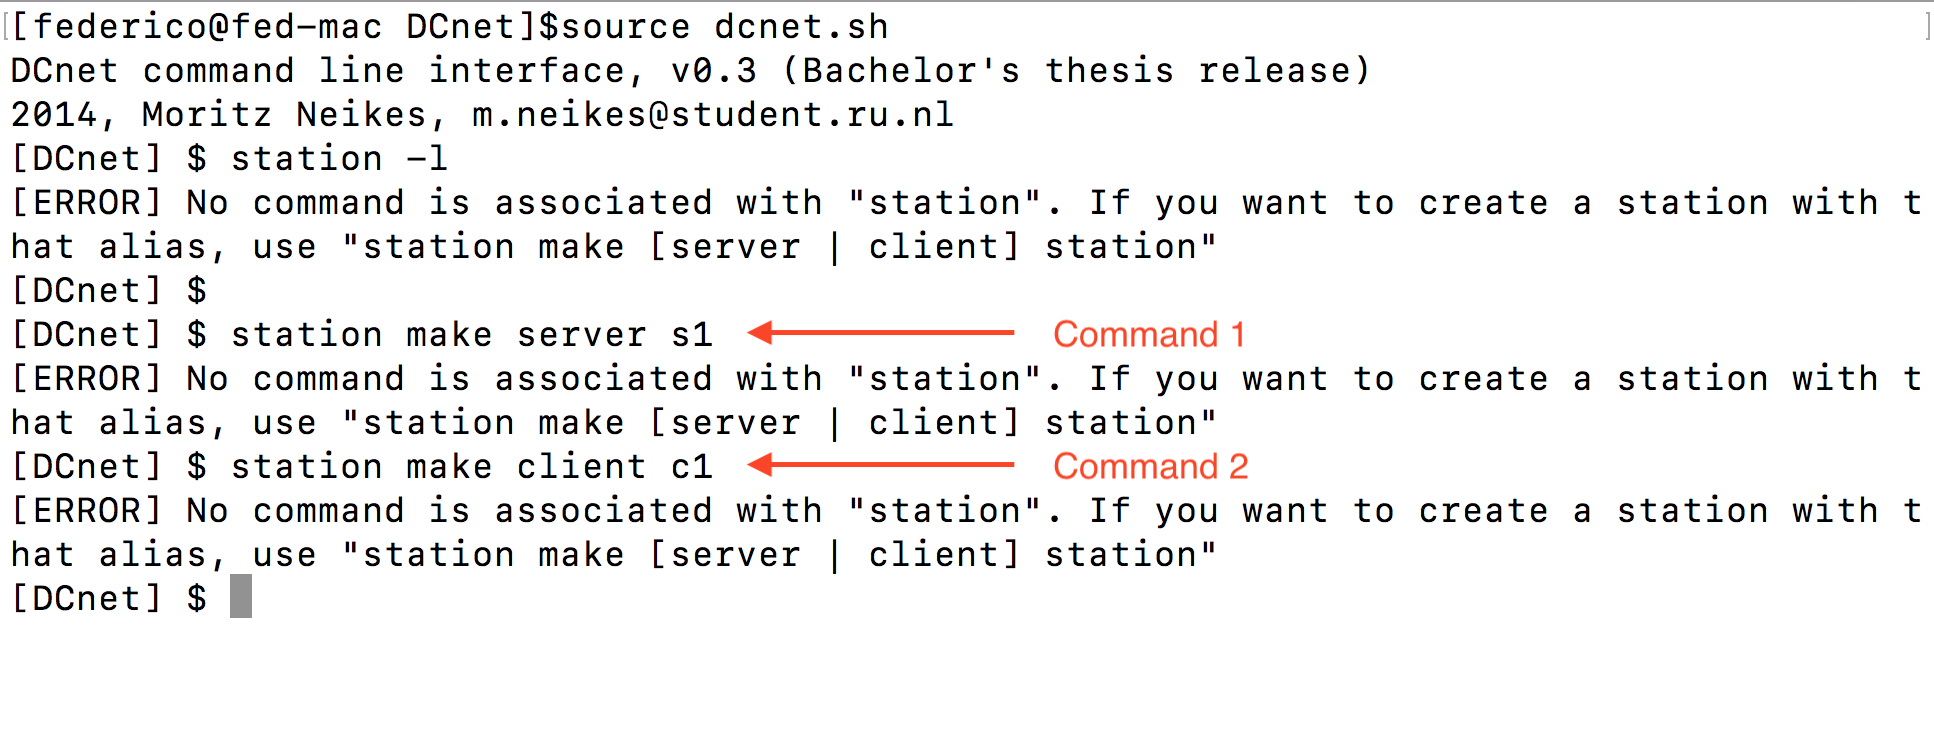
\includegraphics[width=0.7\textwidth]{Images/work1WellDocumentedError.png}
    \caption{Error by following documentation commands.}
    \label{fig:work1error}
\end{figure}

Despite being the best documented project found, there is no setup guide, and the project does not seem to be running in order to solve these issues (last commit over two years ago).

\subsection{Example 2}
Another command line tool found relies on the PubNub as a service to implement the publish subscriber pattern. However, there are no examples of how to configure key files neither on PubNub nor on the documentation of the GitHub project (figure \ref{fig:work2documentation}). Trying to run the software with sample key files results in unhelpful errors(figure \ref{fig:work2error}). 

\begin{figure}[h!]
    \centering
    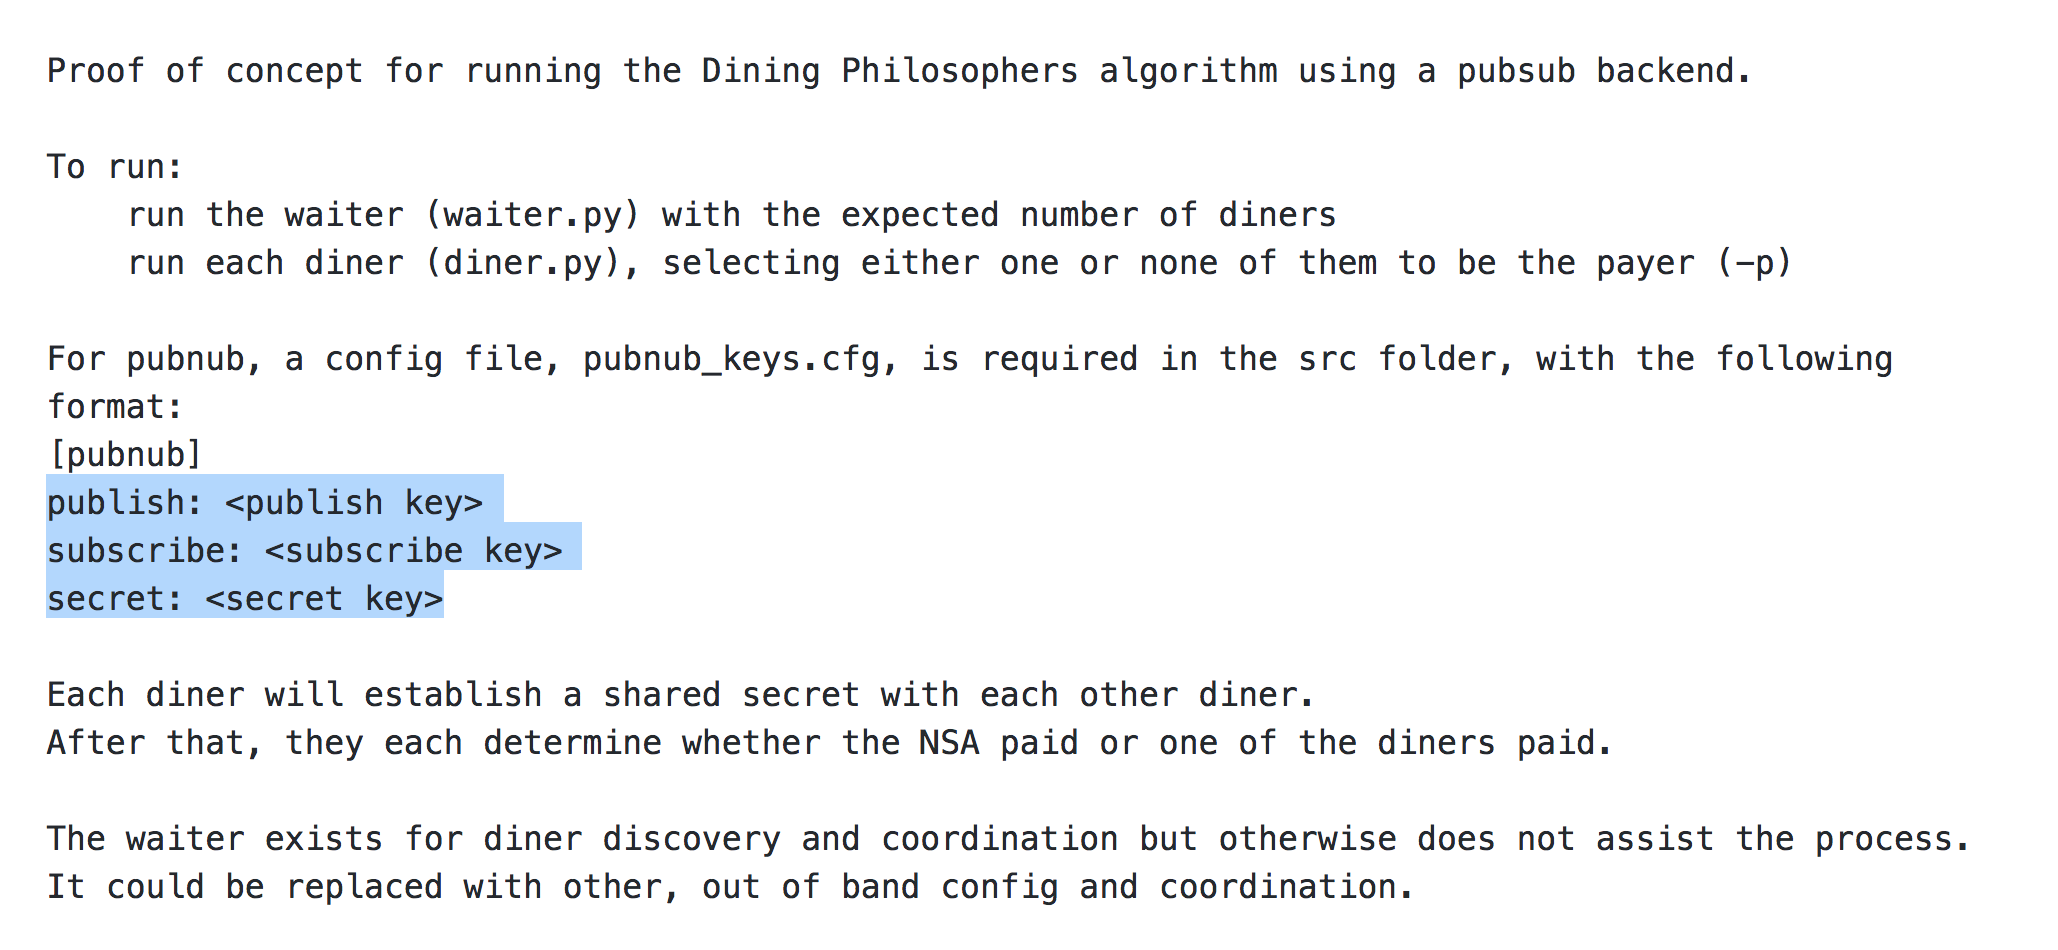
\includegraphics[width=0.7\textwidth]{Images/work2Documentation.png}
    \caption{Documentation instructions but not examples.}
    \label{fig:work2documentation}
\end{figure}

\begin{figure}[h!]
    \centering
    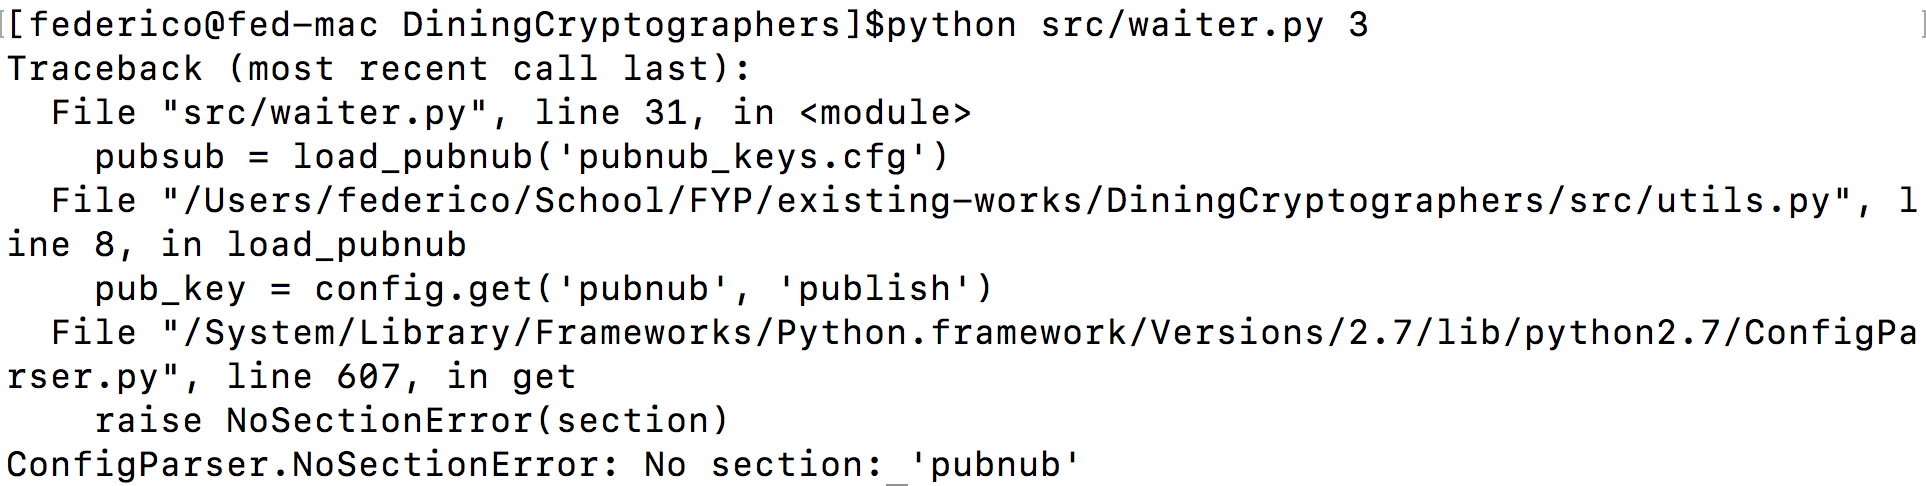
\includegraphics[width=0.7\textwidth]{Images/work2Error.png}
    \caption{Error by trying to run tool with a sample pubnub{\_}keys.cfg.}
    \label{fig:work2error}
\end{figure}

Even if it was to run, this program does not provied a distributed architecture on multiple nodes, so as to resemble closely the multi-party computation.


\subsection{Summary of findings}
The examples shown above were among the best implementations found and they clearly exemplify the lack of practical work on this topic. All projects found are command-line based prototypes. Many of these either present no documentation whatsoever, or do not address fundamental aspects, such as collision detection, in order to encourage a satisfactory discussion for the realistic implementation of a DC-Net. None of them seems to be usable over an actual network, so as to allow multiple users to carry out the protocol.

In the light of these findings, a simulation tool that both illustrates the protocol and investigates the implementations roadblocks is called for.

